%convert -coalesce launch.gif launch_%d.png
\documentclass{beamer}

\newcommand{\VEV}[1]{\langle#1\rangle}
\newcommand{\sst}{\left(1-\frac{2M}{r}\right)}
\newcommand{\sh}{\mathrm{shell}}
\newcommand{\be}{\begin{equation}}
\newcommand{\ee}{\end{equation}}
\newcommand{\bue}{\begin{equation}}
\newcommand{\eue}{\end{equation}}
\newcommand{\bc}{\begin{center}}
\newcommand{\ec}{\end{center}}
\newcommand{\bea}[1]{\begin{eqnarray}\label{#1}}
\newcommand{\eea}{\end{eqnarray}}
\newcommand{\bua}{\begin{eqnarray*}}
\newcommand{\eua}{\end{eqnarray*}}
\newcommand{\dd}[2]{{{d#1}\over{d#2}}}
\newcommand{\ddt}[1]{\dd{#1}{t}}
\newcommand{\dddt}[1]{\dd{^2#1}{t^2}}
\newcommand{\aver}[1]{\langle{#1}\rangle}
\newcommand{\atom}[3]{\ifmmode^{#1}_{#2}{\rm{#3}}\else{$^{#1}_{#2}${#3}}\fi}
\newcommand{\electron}{\atom{~0}{-1}{e}}
\newcommand{\positron}{\atom{0}{0}{\bar{e}}}
\newcommand{\neutrino}{\atom{0}{0}{\nu_e}}
\newcommand{\photon}{\atom{0}{0}{\gamma}}
\newcommand{\antineutrino}{\atom{0}{0}{\bar{\nu}}}
\newcommand{\neutron}{\atom{1}{0}{n}}
\newcommand{\proton}{\atom{1}{1}{p}}
\newcommand{\hydrogen}{\atom{1}{1}{H}}
\newcommand{\deuterium}{\atom{2}{1}{H}}
\newcommand{\tritium}{\atom{3}{1}{H}}
\newcommand{\helium}{\atom{4}{2}{He}}
\newcommand{\hethree}{\atom{3}{2}{He}}

\renewcommand{\ss}{Schwarz\-schild }

\def\densu{kg/m$^3$} 
\def\rsol{R$_{\odot}$} 
\def\msol{M$_{\odot}$} 


\usetheme{Boadilla}
%\usepackage{multimedia}
%\usepackage{animate}
\usepackage{hyperref}
\usepackage{tikz}
\usepackage{cancel}
\usepackage{tikzsymbols}
\usepackage{ifthen}

%%%%mathcircled
\makeatletter
\newcommand\mathcircled[1]{%`
  \mathpalette\@mathcircled{#1}%
}
\newcommand\@mathcircled[2]{%
  \tikz[baseline=(math.base)] \node[draw,circle,red, thick, inner sep=2pt] (math) {$\m@th#1#2$};%
}
\makeatother
%%%%

%gets rid of bottom navigation bars
\setbeamertemplate{footline}[frame number]{} %begin

%gets rid of bottom navigation symbols
\setbeamertemplate{navigation symbols}{}

%gets rid of footer
%will override 'frame number' instruction above  %begin
%comment out to revert to previous/default definitions
\setbeamertemplate{footline}{}

\definecolor{darkscarlet}{rgb}{0.34, 0.01, 0.1}
\definecolor{gold(metallic)}{rgb}{0.83, 0.69, 0.22}
\definecolor{green(ryb)}{rgb}{0.4, 0.69, 0.2}
\definecolor{darkorange}{rgb}{1.0, 0.55, 0.0}
\definecolor{amber}{rgb}{1.0, 0.75, 0.0}
\definecolor{bronze}{rgb}{0.8, 0.5, 0.2}
\definecolor{cadet}{rgb}{0.33, 0.41, 0.47}
\definecolor{silver}{rgb}{0.75, 0.75, 0.75}
\definecolor{turquoise}{rgb}{0.19, 0.84, 0.78}
\definecolor{uclagold}{rgb}{1.0, 0.7, 0.0}
\definecolor{urobilin}{rgb}{0.88, 0.68, 0.13}
\definecolor{vegasgold}{rgb}{0.77, 0.7, 0.35}
\definecolor{vanilla}{rgb}{0.95, 0.9, 0.67}
\definecolor{straw}{rgb}{0.89, 0.85, 0.44}
\definecolor{sunset}{rgb}{0.98, 0.84, 0.65}
\definecolor{brown(traditional)}{rgb}{0.59, 0.29, 0.0}
\definecolor{apricot}{rgb}{0.98, 0.81, 0.69}
\definecolor{darkblue}{rgb}{0,0,0.54}

\hypersetup{
    colorlinks=true,
    linkcolor=yellow,
    filecolor=magenta,
    urlcolor=blue,
}

\let\hrefori\href
\renewcommand{\href}[2]{{\setlength{\fboxsep}{1pt}\colorbox{sunset}{\hrefori{#1}{#2}}}}


%title
\setbeamercolor{block title alerted}{fg=white,bg=cyan}
%body
\setbeamercolor{block body alerted}{fg=black!90,bg=yellow!60}

%title
\setbeamercolor{block title}{fg=black,bg=turquoise}
%body
\setbeamercolor{block body}{fg=yellow,bg=bronze}




\newcommand{\pagebutton}[1]{\setbeamertemplate{button}{\tikz\node[inner xsep = 5pt, draw = structure!90, fill = green(ryb), rounded corners = 8pt]{\color{amber}\Large\insertbuttontext};}\beamerbutton{#1}}

\newcommand{\choicebutton}[1]{\setbeamertemplate{button}{\tikz\node[inner xsep = 8pt, draw = structure!90, fill = vegasgold, rounded corners = 5pt]{\color{vanilla}\Large\insertbuttontext};}\beamerbutton{#1}}

\newcommand{\pagenobutton}[1]{\setbeamertemplate{button}{\tikz\node[inner xsep = 8pt, draw = structure!90, fill = apricot, rounded corners = 5pt]{\color{brown(traditional)}\Large\insertbuttontext};}\beamerbutton{#1}}

\newcommand{\headlinebutton}[1]{\setbeamertemplate{button}{\tikz\node[inner xsep = 8pt, draw = structure!90, fill = blue, rounded corners = 5pt]{\color{yellow}\Large\insertbuttontext};}\beamerbutton{#1}}

\newcommand{\forumbutton}{\href{https://astro-discourse.utenforuio.no/c/ast2000/sporsmal-til-ukeoppgavene-i-del-2a-2d/11}{\setbeamertemplate{button}{\tikz\node[inner xsep = 8pt, draw = structure!90, fill = darkblue, rounded corners = 5pt]{\color{yellow}\Large\insertbuttontext};}\beamerbutton{\textcolor{red}{\small FORUM}}}}

\newcommand{\curpage}{\pagenobutton{\small side \thepageno\  av \thenopages}}
\newcommand{\nextpage}{\refstepcounter{pageno}\pagenobutton{\small side \thepageno\  av \thenopages}}
\newcommand{\dnextpage}{\refstepcounter{pageno}\refstepcounter{pageno}\pagenobutton{\small side \thepageno\  av \thenopages}}

\newcommand{\lastpagebutton}[1]{\hyperlink{#1}{\pagebutton{\small Forrige side}}\href{https://nettskjema.no/a/171403}{\Changey[1][yellow]{2} \Changey[1][yellow]{-2}}\nextpage\headlinebutton{\headline}\forumbutton}
\newcommand{\clastpagebutton}[1]{\hyperlink{#1}{\pagebutton{\small Forrige side}}\href{https://nettskjema.no/a/171403}{\Changey[1][yellow]{2} \Changey[1][yellow]{-2}}\curpage\headlinebutton{\headline}\forumbutton}
\newcommand{\dlastpagebutton}[1]{\hyperlink{#1}{\pagebutton{\small Forrige side}}\href{https://nettskjema.no/a/171403}{\Changey[1][yellow]{2} \Changey[1][yellow]{-2}}\dnextpage\headlinebutton{\headline}\forumbutton}

\newcommand{\lastpagebuttonx}[1]{\hyperlink{#1}{\pagebutton{\small Forrige side}}\href{https://nettskjema.no/a/171403}{\Changey[1][yellow]{2} \Changey[1][yellow]{-2}}\nextpage\\}
\newcommand{\clastpagebuttonx}[1]{\hyperlink{#1}{\pagebutton{\small Forrige side}}\href{https://nettskjema.no/a/171403}{\Changey[1][yellow]{2} \Changey[1][yellow]{-2}}\curpage\\}
\newcommand{\dlastpagebuttonx}[1]{\hyperlink{#1}{\pagebutton{\small Forrige side}}\href{https://nettskjema.no/a/171403}{\Changey[1][yellow]{2} \Changey[1][yellow]{-2}}\dnextpage\\}

\newcommand{\lastpagebuttoncr}[1]{\hyperlink{#1}{\pagebutton{\small Forrige side}}\href{https://nettskjema.no/a/171403}{\Changey[1][yellow]{2} \Changey[1][yellow]{-2}}\nextpage\\\headlinebutton{\headline}\forumbutton\\}
\newcommand{\clastpagebuttoncr}[1]{\hyperlink{#1}{\pagebutton{\small Forrige side}}\href{https://nettskjema.no/a/171403}{\Changey[1][yellow]{2} \Changey[1][yellow]{-2}}\curpage\\\headlinebutton{\headline}\forumbutton\\}
\newcommand{\dlastpagebuttoncr}[1]{\hyperlink{#1}{\pagebutton{\small Forrige side}}\href{https://nettskjema.no/a/171403}{\Changey[1][yellow]{2} \Changey[1][yellow]{-2}}\dnextpage\\\headlinebutton{\headline}\forumbutton\\}

\newcommand{\nytemaside}[1]{
\centerline{\Huge\textcolor{yellow}{Nytt tema:}}\\
\vspace*{1cm}
\centerline{\Large\bf\textcolor{yellow}{\headline}}
\vspace*{2cm}
\ifthenelse{\equal{#1}{0}}{\centerline{\textcolor{yellow}{Siste tema i denne forelesningen!}}}{\centerline{\textcolor{yellow}{\footnotesize Dette temaet fortsetter frem til side \ref{#1} av \thenopages.}}}
\vspace*{0.5cm}
}


\newcommand{\fullframe}[6]{
\begin{frame}
\label{#1}
\addtocounter{pageno}{#4}
\lastpagebutton{#2}{\bf #6}\\
#5
\hyperlink{#3}{\pagebutton{Neste side}}
\end{frame}
}



\newcommand{\fullframetwo}[7]{
\begin{frame}
\label{#1}
\addtocounter{pageno}{#4}
\lastpagebutton{#2}{\bf #7}\\
\begin{columns}
\column{0.5\textwidth}
#5
\column{0.5\textwidth}
#6
\hyperlink{#3}{\pagebutton{Neste side}}
\end{columns}
\end{frame}
}

\newcommand{\fullframetwonotxt}[7]{
\begin{frame}
\label{#1}
\addtocounter{pageno}{#4}
\lastpagebutton{#2}{\bf #7}\\
\begin{columns}
\column{0.5\textwidth}
#5
\column{0.5\textwidth}
#6
\end{columns}
\end{frame}
}



\newcommand{\fullframetxt}[7]{
\begin{frame}
\label{#1}
\addtocounter{pageno}{#4}
\lastpagebutton{#2}{\bf #7}\\
#6
\hyperlink{#3}{\pagebutton{#5}}
\end{frame}
}

\newcommand{\fullframenotxt}[6]{
\begin{frame}
\label{#1}
\addtocounter{pageno}{#4}
\lastpagebutton{#2}{\bf #6}\\
#5
\end{frame}
}

\newcommand{\choiceframe}[5]{
\begin{frame}
\label{#1}
\addtocounter{pageno}{#3}
\lastpagebutton{#2}{\bf #5}\\
#4
\end{frame}
}

\newcommand{\colfullframe}[7]{
{
\setbeamercolor{background canvas}{bg=#5}
\begin{frame}
\label{#1}
\addtocounter{pageno}{#4}
\lastpagebutton{#2}{\bf #7}\\
#6
\hyperlink{#3}{\pagebutton{Neste side}}
\end{frame}
}
}

\newcommand{\colfullframetwo}[8]{
{
\setbeamercolor{background canvas}{bg=#5}
\begin{frame}
\label{#1}
\addtocounter{pageno}{#4}
\lastpagebutton{#2}{\bf #8}\\
\begin{columns}
\column{0.5\textwidth}
#6
\column{0.5\textwidth}
#7
\hyperlink{#3}{\pagebutton{Neste side}}
\end{columns}
\end{frame}
}
}

\newcommand{\colfullframetxt}[8]{
{
\setbeamercolor{background canvas}{bg=#5}
\begin{frame}
\label{#1}
\addtocounter{pageno}{#4}
\lastpagebutton{#2}{\bf #8}\\
#7
\hyperlink{#3}{\pagebutton{#6}}
\end{frame}
}
}

\newcommand{\colchoiceframe}[6]{
{
\setbeamercolor{background canvas}{bg=#4}
\begin{frame}
\label{#1}
\addtocounter{pageno}{#3}
\lastpagebutton{#2}{\bf #6}\\
#5
\end{frame}
}
}


\newcommand{\pagequestion}[3]{
\hyperlink{#1}{\pagebutton{#2}}
\pause
%#3 normalt -1 for første spørsmål
\addtocounter{pageno}{#3}
\begin{itemize}[<+->]
\item[] \hypertarget<.>{#1}{}
\end{itemize}
\vspace{-0.5cm}
}

\newcommand{\samepagequestion}[4]{
\hyperlink{#1}{\pagebutton{#2}}\hyperlink{#1}{\pagebutton{#3}}
\pause
%#3 normalt -1 for første spørsmål
\addtocounter{pageno}{#4}
\begin{itemize}[<+->]
\item[] \hypertarget<.>{#1}{}
\end{itemize}
\vspace{-0.5cm}
}

\newcommand{\twopagequestion}[7]{
\hyperlink{#1}{\pagebutton{#3}}\hyperlink{#2}{\pagebutton{#4}}
\pause
%#3 normalt -1 for første spørsmål
\addtocounter{pageno}{#5}
\begin{itemize}[<+->]
\item[] \hypertarget<.>{#1}{}
\end{itemize}
\vspace{-0.5cm}
#7
\addtocounter{pageno}{#6}
\begin{itemize}[<+->]
\item[] \hypertarget<.>{#1}{}
\end{itemize}
\vspace{-0.5cm}
}

\newcounter{pageno}
\newcounter{nopages}
\setcounter{nopages}{42}

\newcommand{\headline}{\small Introduksjon}
\newcommand{\m}{\mathrm{m}}

\begin{document}

\begin{frame}
\label{front2}
\center{\Large \textcolor{darkscarlet}{\bf AST2000 Del 2B\\Interaktive forelesningsnotater: forelesning 2 av 2}}\\
\begin{block}{\center{\bf VIKTIG}}
\textcolor{yellow}{Dette er et alternativ til forelesningen i emnet.} \textcolor{blue}{Har du gått skikkelig gjennom disse interaktive forelesningsnotatene så trenger du ikke å lese \href{https://www.uio.no/studier/emner/matnat/astro/AST2000/h21/undervisningsmateriell/lecture_notes/part2b.pdf}{de fulle forelesningsnotatene} (med unntak av oppgavene bak)}. All informasjonen du trenger, får du her. Du kommer til å få mange grublespørsmål og diskusjonsoppgaver, det er meningen at disse skal gjøres i grupper av minst 2, maks 4 studenter. {\bf Det er defor sterkt anbefalt at dere sitter sammen i grupper når dere går gjennom disse interaktive forelesningsnotatene, du vil få betydelig mer utbytte av dem på den måten}. {\bf Hvis du har kommentarer ris/ros til disse forelesningsnotatene eller til emnet, trykk på \href{https://nettskjema.no/a/171403}{\Changey[1][yellow]{2} \Changey[1][yellow]{-2}}\ knappen som du finner på alle sider.}
\end{block}
%\setbeamercolor{button}{bg=black,fg=yellow}
\hyperlink{front3}{\pagebutton{Trykk denne knappen for å begynne}}
\end{frame}

\begin{frame}
\label{front3}
{\Large
\begin{itemize}
\item HUSK at du får mer ut av de interaktive forelesningsnotatene når du gjør de sammen med noen. Diskusjonene med andre er svært viktige.
\item Det er mange spørsmål/grubliser underveis, sett dere selv en tidsgrense, 1 minutt på de korte, maks 4-5 minutter på de lenger. Ha en alarm ved siden av, ellers kommer dere til å bruke alt for langt tid. Har dere ikke fått det til etter kort tid, gå videre, se svaret og lær!
\item Er du i det minste tvil om noe, så finnes det en \forumbutton knapp, trykk det og still spørsmål med en gang mens du enda husker spørsmålet!
\end{itemize}
}
\hyperlink{tableofcontents}{\pagebutton{Trykk denne knappen for å begynne}}
\end{frame}

\begin{frame}
\label{tableofcontents}
\hyperlink{front3}{\pagebutton{Forrige side}}\\
Hvis du allerede har begynt på denne forelesningen og vil hoppe rett inn til et annet kapittel, kan du trykke her:
\begin{itemize}
\item \hyperlink{blue_nytema1}{\headlinebutton{Regneregler for 4-vektorer}}
\item \hyperlink{blue_nytema2}{\headlinebutton{4-hastighet}}
\item \hyperlink{hast9}{\headlinebutton{Tolkning av 4-hastighet}}
\item \hyperlink{blue_nytema3}{\headlinebutton{Hastighetstransformasjoner}}
\item \hyperlink{blue_nytema4}{\headlinebutton{Relativistisk begevelsesmengde}}
\item \hyperlink{pe8}{\headlinebutton{Relativistisk energi}}
\item \hyperlink{pe17b}{\headlinebutton{Kjernereaksjoner}}
\end{itemize}
Merk at sidene er merket med sidenummer på denne måten: SIDE X/Y/Z. Her er Z antall sider totalt, Y er sidenummeret til siste side i avsnittet du holder på med og X er sidenummeret til siden du er på.\\
\hyperlink{intro}{\choicebutton{Neste side}}
\end{frame}

%%%%% intro
\begin{frame}
\label{intro}
\begin{columns}
\column{0.5\textwidth}
\hyperlink{front3}{\pagebutton{Forrige side}}\\

\includegraphics[scale=0.25]{media/clock.png}
\column{0.5\textwidth}
{\small
{\bf Velkommen til forelesning 2 av 2 i del 2B! I denne forelesningen skal vi gå gjennom eksempler der vi bruker tidromsintervallets invarians til å løse forskjellige problemstillinger. Disse problemstillingene likner mye på de som du trenger å løse for prosjektet eller for eksamen, så følg nøye med. }\\
\textcolor{red}{Fremstillingen av spesiell relativitetsteori i AST2000 er basert på den fantastiske boken ``Spacetime Physics'' av E. Taylor og J. Wheeler, gratis tilgjengelig \href{http://www.eftaylor.com/spacetimephysics/}{her}. Anbefales på det sterkeste for den som er interessert.}
{(\tiny Illustrasjon fra pngegg.com)}}
\hyperlink{intro2}{\pagebutton{Neste side}}
\end{columns}
\end{frame}



\begin{frame}`
\label{intro2}
\lastpagebutton{intro}
\begin{alertblock}{Vi begynner som vanlig...}
...med litt brainstorming. Som det er {\bf svært viktig} at du gjør før du går videre.
\end{alertblock}
\href{https://nettskjema.no/a/171389}{\begin{minipage}{5cm}Trykk her for å varme opp\end{minipage}}\\
Er du klar og har sendt inn skjemaet?
\href{https://nettskjema.no/a/171389}{\choicebutton{Nei}}\ \ \ \ \hyperlink{blue_nytema1}{\choicebutton{Ja}}\\
\end{frame}



\renewcommand{\headline}{\small Regneregler for 4-vektorer}
{
\setbeamercolor{background canvas}{bg=blue}
\begin{frame}
\label{blue_nytema1}
\hyperlink{intro2}{\pagebutton{\small Forrige side}}
\nytemaside{hast}
\hyperlink{vv1}{\pagebutton{Sett igang!}}
\end{frame}
}

\fullframe{vv1}{intro2}{vv2}{1}{\Huge
Vi begynner med en oppsummering av det vi vet om 4-vektorer i \href{https://www.uio.no/studier/emner/matnat/astro/AST2000/h20/undervisningsmateriell/interaktive-forelesningsnotater/2b/videoer/video2b_13.mp4}{denne videoen}
}{SIDE 1/10/56}

\fullframetxt{vv2}{vv1}{red_vv3}{0}{\small Trykk her etter at du har tenkt gjennom hva en 4-vektor er}{\large
Vi skal utlede litt regneregler for 4-vektorer. {\bf Det som er spesielt viktig for å vite om en regneoperasjon på en 4-vektor er lov, er om resultatet av regneoperasjonen også er en 4-vektor.} \textcolor{red}{La oss si at du har en 4-vektor $A_\mu$. Og så har du et tidromsintervall $\Delta s$ mellom to eventer.} Si at du av en eller annen grunn skal \textcolor{red}{gange dette tidromsintervallet med 4-vektoren $A_\mu$.}{\Huge Kan du gjøre det????} {\bf Eller rettere sagt: blir resultatet av denne gangeoperasjonen en 4-vektor?} Sagt matematisk:
\[
B_\mu=\Delta s A_\mu
\]
Er $B_\mu$ en 4-vektor? Hvordan kan vi sjekke det?
}{SIDE 2/10/56}


\colfullframe{red_vv3}{vv2}{vv4}{0}{red}{\Huge
\textcolor{yellow}{Så? {\bf Er} $B_\mu$ virkelig en 4-vektor eller ikke? Hva var kravet til en 4-vektor? Er du usikker, gå tilbake til repetisjonen i starten her.}
}{SIDE 3/10/56}

\fullframetxt{vv4}{red_vv3}{red_vv5}{0}{Jeg har tenkt godt gjennom problemstillingen}{\Large
Er ikke kravet at en 4-vektor skal kunne transformeres fra et referansesystem til et annet med Lorentz-transformasjonen? Vi vet at $A_\mu$ er en 4-vektor, så for denne vet vi at
\[
A_\mu'=C_{\mu\nu}A_\nu
\]
er oppfylt (merk, $C_{\mu\nu}$ er Lorentzmatrisa og Einsteins summekonvensjon har blitt brukt). Dermed vet vi hva komponentene av $A_\mu$ er i det merkede systemet, hvis vi kjenner dem i det umerkede. {\Huge Men oppfyller $B_\mu$ denne betingelsen?}
}{SIDE 4/10/56}

\colfullframe{red_vv5}{vv4}{vv6}{0}{red}{\Large
\textcolor{yellow}{Det holder ikke bare å ha tenkte godt gjennom problemstillingen her, denne bør du nå ha nok informasjon til å kunne vise matematisk. Men la gå da, noen tips til: Du vet at $B_\mu=\Delta s A_\mu$. Prøv å finne ut hvordan $B_\mu'$ ser ut. Du vet hvordan både $A_\mu$ og $\Delta s$ (ja det vet du!) transformerer til merket system. Anta at $B_\mu'=\Delta s'A_\mu'$. Følger $B_\mu$ Lorentztransformasjonen og er dermed en 4-vektor eller ikke??}
}{SIDE 5/10/56}



\fullframe{vv6}{red_vv5}{vv6b}{0}{\Huge
Klarte du å vise at
\[
B_\mu'=C_{\mu\nu}B_\nu
\]
og at $B_\mu$ dermed er en 4-vektor?? Hvis ikke, ta en titt på \href{https://www.uio.no/studier/emner/matnat/astro/AST2000/h20/undervisningsmateriell/interaktive-forelesningsnotater/2b/videoer/video2b_14.mp4}{denne videoen}
\textcolor{red}{Vi har vist at vi kan gange en 4-vektor med et tidromsintervall $\Delta s$!}
}{SIDE 6/10/56}

\fullframe{vv6b}{vv6}{vv6c}{0}{\huge
La oss ta en til: Hvis vi nå isteden for å gange $A_\mu$ med $\Delta s$, ganger $A_\mu$ med et tidspunkt $t$ for et event. Altså si at du prøver å lage en 4-vektor $B_\mu$ på denne måten:
\[
B_\mu=tA_\mu
\]
der $t$ er tidspunktet til et event målt i umerket system. {\Huge Er $B_\mu$ en 4-vektor?} Gjenta utledningen du akkurat gjorde på nytt...
}{SIDE 7/10/56}


\fullframe{vv6c}{vv6b}{vv7}{0}{\huge
Fant du at $B_\mu$ {\bf IKKE} er en 4-vektor i dette tilfellet? At vi derfor {\bf ikke} kan gange 4-vektorer med tidspunkter? Fordi vi da ikke lenger får en 4-vektor tilbake? Er du usikker, ta en titt på \href{https://www.uio.no/studier/emner/matnat/astro/AST2000/h20/undervisningsmateriell/interaktive-forelesningsnotater/2b/videoer/video2b_15.mp4}{denne videoen}.
}{SIDE 8/10/56}

\fullframe{vv7}{vv6c}{vv8}{0}{\Large
  Vi har altså vist at vi fint kan gange en 4-vektor med en {\bf invariant} størrelse, eller en {\bf skalar}. I relativitetsteorien kaller vi invariante størrelser for skalarer. Tidromsintervallet $\Delta s$ er et eksempel på en slik skalar. Vi så at $B_\mu$ ble en 4-vektor nettopp fordi $\Delta s$ er invariant. I det vi prøvde å gange $A_\mu$ med en størrelse som ikke er invariant, slik som et tidspunkt $t$ (som jo har forskjellig verdi i forskjellige referansesystemer) så fikk vi ikke en 4-vektor tilbake.
}{SIDE 9/10/56}

\fullframe{vv8}{vv7}{blue_nytema2}{0}{\huge
  Vi har altså lært at vi kan gange 4-vektorer med skalarer, men {\bf ikke med en hvilken som helst størrelse}. Det samme gjelder deling, du kan gjøre akkurat de samme bevisene og vise at vi kan dele 4-vektorer med skalarer men ikke med tall som ikke er invariante! I ukeoppgavene skal du vise at vi kan plusse og trekke 4-vektorer fra hverandre akkurat som med vanlige vektorer
}{SIDE 10/10/56}


\renewcommand{\headline}{4-hastighet}
{
\setbeamercolor{background canvas}{bg=blue}
\begin{frame}
\label{blue_nytema2}
\hyperlink{vv8}{\pagebutton{\small Forrige side}}
\nytemaside{htrans}
\hyperlink{hast1}{\pagebutton{Hvor fort går jeg i tidrommet?}}
\end{frame}
}

\fullframetxt{hast1}{vv8}{hast2}{0}{jeg har et forslag}{\label{hast}\Large
Hvis vi har en posisjonsvektor $\vec{x}$ for et objekt, så vet vi at hastigheten til dette objektet er gitt ved
\[
\vec{v}=\frac{d\vec{x}}{dt}.
\]
Kan vi definere en tilsvarende 4-dimensjonal hastighet? Altså med hvilken hastighet beveger du deg gjennom tidrommet? Posisjonen din i rom og tid kan vi angi med en posisjons-4-vektor $x_\mu$.{\Huge Men hva blir 4-hastigheten din, $V_\mu$?} Noen forslag til hvordan denne kan defineres?
}{SIDE 11/26/56}

\choiceframe{hast2}{hast1}{0}{\huge
Fikk du:
\[
V_\mu=\frac{dx_\mu}{dt}
\]
\hyperlink{feil_hast2b}{\choicebutton{det høres ut som en fornuftig generalisering...}}
\hyperlink{feil_hast2a}{\choicebutton{Næææææææ.....}}
}{SIDE 12/26/56}

\colfullframe{feil_hast2a}{hast2}{feil_hast3}{0}{black}{\Huge
\textcolor{yellow}{Du har god grunn til å tvile ja, men {\bf hvilken grunn?} Ikke gå videre før du vet hvorfor du tviler! Se på uttrykket en gang til:
\[
V_\mu=\frac{dx_\mu}{dt}
\]
Hva er galt her? (hva lært vi nettopp?)
}
}{SIDE 13/26/56}

\colfullframe{feil_hast2b}{hast2}{feil_hast3}{-1}{black}{\Huge
\textcolor{yellow}{Fornuftig sier du? Se på uttrykket en gang til:
\[
V_\mu=\frac{dx_\mu}{dt}
\]
Hva er galt her? (hva lærte vi nettopp?)}
}{SIDE 14/26/56}

\colfullframe{feil_hast3}{hast2}{red_hast4}{0}{black}{\Large
\textcolor{yellow}{
\[
V_\mu=\frac{dx_\mu}{dt}
\]
Vi ser her at $dx_\mu$ er en 4-vektor (en differanse $\Delta x_\mu$ mellom to eventer eller to punkter langs verdenslinja) men $dt$ er {\bf ikke en skalar!}. Vi utledet over at vi ikke kan gange/dele en 4-vektor med et tall som ikke er en skalar! $dt$ er et tidsintervall målt i et gitt referansesystem. Dette tallet er forskjellig i et annet referansesystem. Dermed blir {\bf ikke} $V_\mu$ en 4-vektor. Og hvis vi vil ha en hastighetsvektor i det 4-dimensjonale rom, bør det være en 4-vektor! \textcolor{red}{\Huge Har du et bedre forslag?}}
}{SIDE 15/26/56}


\colfullframe{red_hast4}{feil_hast3}{hast5}{0}{red}{\Huge
  Et hint: kan vi derivere med hensyn på {\bf en annen tid} enn $t$? Ikke bla videre før du har et forslag!
}{SIDE 16/26/56}

\fullframenotxt{hast5}{red_hast4}{red_hast6}{0}{
  Hva med {\bf egentid $\tau$? Husker du hva det var?}\hyperlink{hast5_b}{\pagebutton{javisst ja (evt. jeg repeterte nå)}}\\
  \textcolor{white}{
Var ikke det armbåndsurtid?{jovisst!}\\
Altså tiden målt på en klokke som står fast på objektet som vi ser på, altså det objektet vi måler hastigheten til. Men er det en invariant størrelse da? ({\bf det må del vel være for at vi skal dele det med en 4-vektor!?)}{det var det og jeg husker hvorfor (evt. jeg repeterte nå)}\\
Viste ikke vi i forrige forelesning at $\Delta s = \Delta \tau$? Og hvis $\Delta s$ er invariant så må også $\Delta \tau$ altså egentidsintervaller, være det. Men kan du se intuitivt hvorfor et egentidsintervall er invariant? Hvor bare {\bf må} det per def være en invariant størrelse?}
}{SIDE 17/26/56}

\fullframenotxt{hast5_b}{red_hast4}{red_hast6}{0}{
Hva med {\bf egentid $\tau$? Husker du hva det var?}\pagebutton{javisst ja (evt. jeg repeterte nå)}\\
Var ikke det armbåndsurtid?\hyperlink{hast5_c}{\pagebutton{jovisst!}}\\
\textcolor{white}{
Altså tiden målt på en klokke som står fast på objektet som vi ser på, altså det objektet vi måler hastigheten til. Men er det en invariant størrelse da? ({\bf det må del vel være for at vi skal dele det med en 4-vektor!?)}{det var det og jeg husker hvorfor (evt. jeg repeterte nå)}\\
Viste ikke vi i forrige forelesning at $\Delta s = \Delta \tau$? Og hvis $\Delta s$ er invariant så må også $\Delta \tau$ altså egentidsintervaller, være det. Men kan du se intuitivt hvorfor et egentidsintervall er invariant? Hvor bare {\bf må} det per def være en invariant størrelse?}
}{SIDE 17/26/56}

\fullframenotxt{hast5_c}{red_hast4}{red_hast6}{0}{
Hva med {\bf egentid $\tau$? Husker du hva det var?}\pagebutton{javisst ja (evt. jeg repeterte nå)}\\
Var ikke det armbåndsurtid?{\pagebutton{jovisst!}}\\
Altså tiden målt på en klokke som står fast på objektet som vi ser på, altså det objektet vi måler hastigheten til. Men er det en invariant størrelse da? ({\bf det må del vel være for at vi skal dele det med en 4-vektor!?)}\hyperlink{hast5_d}{\pagebutton{det var det og jeg husker hvorfor (evt. jeg repeterte nå)}}\\
\textcolor{white}{
Viste ikke vi i forrige forelesning at $\Delta s = \Delta \tau$? Og hvis $\Delta s$ er invariant så må også $\Delta \tau$ altså egentidsintervaller, være det. Men kan du se intuitivt hvorfor et egentidsintervall er invariant? Hvor bare {\bf må} det per def være en invariant størrelse?}
}{SIDE 17/26/56}

\fullframetxt{hast5_d}{red_hast4}{red_hast6}{0}{Dette bør du kunne svare på}{
Hva med {\bf egentid $\tau$? Husker du hva det var?}\pagebutton{javisst ja (evt. jeg repeterte nå)}\\
Var ikke det armbåndsurtid?{\pagebutton{jovisst!}}\\
Altså tiden målt på en klokke som står fast på objektet som vi ser på, altså det objektet vi måler hastigheten til. Men er det en invariant størrelse da? ({\bf det må del vel være for at vi skal dele det med en 4-vektor!?)}{\pagebutton{det var det og jeg husker hvorfor (evt. jeg repeterte nå)}}\\
Viste ikke vi i forrige forelesning at $\Delta s = \Delta \tau$? Og hvis $\Delta s$ er invariant så må også $\Delta \tau$ altså egentidsintervaller, være det. Men kan du se intuitivt hvorfor et egentidsintervall er invariant? Hvorfor bare {\bf må} det per def være en invariant størrelse?
}{SIDE 17/26/56}











\colfullframe{red_hast6}{hast5}{hast7}{1}{red}{\Huge
  Et hint: hva betyr invariant? Dette {\bf må} du ha kontroll på nå, hvis ikke spør!
}{SIDE 18/26/56}

\fullframe{hast7}{red_hast6}{hast8}{0}{\huge
Egentid er jo per def tiden målt på klokka til objektet som vi ser på {\bf og på ingen annen klokke}. Det betyr at egentiden $\tau$ er den tiden som alle observatører i alle referansesystemer leser av (kanskje med kikkert) på klokka som står fast på objektet. {\bf Dermed må alle observatører være enige i denne tiden siden alle leser den av på den samme klokka!}
}{SIDE 19/26/56}

\fullframe{hast8}{hast7}{hast9}{0}{\huge
Da må vi altså ha følgende definisjon av 4-hastighet:
\[
V_\mu=\frac{dx_\mu}{d\tau}
\]
4-hastighet er endring i tidromsposisjon $x_\mu$ målt av en gitt observatør (denne størrelsen vil avhenge av observatøren som måler) delt på egentiden $\Delta\tau$ det tar for denne endringen å finne sted (målt på klokka på objektet!).
}{SIDE 20/26/56}

\fullframe{hast9}{hast8}{hast10}{0}{\Large
OK, la oss se om vi kan skrive ut 4-hastigheten litt mer her. En posisjonsvektor $x_\mu$ i tidrommet kan vi skrive ut på komponentform som
\[
x_\mu=(t,x,y,z)
\]
Enig? Og siden $V_\mu=\frac{dx_\mu}{d\tau}$ så skal vi derivere hver og en komponent av $x_\mu$ med hensyn på egentid $\tau$. Kan du vise at du etter bittelitt regning kan skrive dette som:
\[
V_\mu=\frac{dt}{d\tau}(1,v_x,v_y,v_z)
\]
der $t$ er tiden målt i det samme referansesystemet som måler posisjonsvektoren $x_\mu$, og hastighetskomponentene er hastighet også målt i dette referansesystemet? (bruk maks 3 min)
}{SIDE 21/26/56}


\fullframe{hast10}{hast9}{hast11}{0}{\Large
Hvis du ikke fikk det til, se på \href{https://www.uio.no/studier/emner/matnat/astro/AST2000/h20/undervisningsmateriell/interaktive-forelesningsnotater/2b/videoer/video2b_16.mp4}{denne videoen}. Kan du videre vise at
\[
V_\mu=\gamma(1,\vec{v})
\]
der
\[
\gamma=\frac{1}{\sqrt{1-v^2}}
\]
der $v$ er fart målt i det samme referansesystemet som måler posisjonsvektoren $x_\mu$? Og $\vec{v}$ er rett og slett den 3-dimensjonale hastighetsvektoren også målt i dette referansesystemet. (bruk maks 2 min)
}{SIDE 22/26/56}

\fullframe{hast11}{hast10}{pause}{0}{\Large
Hvis du ikke fikk det til, se på \href{https://www.uio.no/studier/emner/matnat/astro/AST2000/h20/undervisningsmateriell/interaktive-forelesningsnotater/2b/videoer/video2b_17.mp4}{denne videoen}.
}{SIDE 23/26/56}


{
\setbeamercolor{background canvas}{bg=cyan}
\begin{frame}
\label{pause}
\hyperlink{hast11}{\pagebutton{\small Forrige side}}
{\huge
\centerline{Kaffe!}
\centerline{
\includegraphics[scale=4]{media/drink-coffee.png}}\\
Kanskje skulle du legge deg ned på sofaen og lukke øynene i 10 min? Så alt ikke helt går i surr! Og så en strekk på bena, ok ikke minst {\bf kaffe!}.
}\\
\vspace*{0.5cm}
\hyperlink{hast12}{\pagebutton{Jeg er klar til å fortsette...}}
\end{frame}
}



\fullframe{hast12}{hast11}{hast13}{0}{\large
Vi kan altså skrive 4-hastighet som:
\[
V_\mu=\gamma(1,\vec{v})=(\gamma, \gamma\vec{v})
\]
Vi ser at {\bf tidsdelen} av 4-vektoren, altså den første komponenten i 4-vektoren (som for posisjons-4-vektorer er tiden), her er kun Lorentzfaktoren $\gamma$. Mens {\bf den romlige delen} av 4-vektoren  (som for posisjons-4-vektorer er posisjonen) er hastighet ganger Lorentzfaktoren. Som for vanlige 3D-vektorer så kan vi finne lengden av en vektor ved å ta skalarproduktet av vektoren med seg selv. Vi kan altså finne 4-farten ved å gjøre nettopp dette med 4-hastighetsvektor:
\[
V=\sqrt{V_\mu V^\mu}
\]
Merk deg en $\mu$-indeks er nede og en er oppe for å indikere {\bf skalarprodukt.} \textcolor{red}{Husker du hvordan man beregner skalarproduktet?} Gjør et forsøk nå på å finne en verdi for $V$! (maks 2 min)
}{SIDE 24/26/56}

\fullframe{hast13}{hast12}{hast14}{0}{\Large
Fikk du...
\[
V=\sqrt{V_\mu V^\mu}=1
\]
????
Hvis ikke, ta en titt på \href{https://www.uio.no/studier/emner/matnat/astro/AST2000/h20/undervisningsmateriell/interaktive-forelesningsnotater/2b/videoer/video2b_18.mp4}{denne videoen}.
}{SIDE 25/26/56}

\fullframe{hast14}{hast13}{blue_nytema2b}{0}{\Huge
Hvordan kan vi tolke dette??? En fart på 1 betyr lysfarta? Beveger vi oss alle med lysfarta gjennom tidrommet? I \href{https://www.uio.no/studier/emner/matnat/astro/AST2000/h20/undervisningsmateriell/interaktive-forelesningsnotater/2b/videoer/video2b_19.mp4}{denne videoen} får du en tolkning.
}{SIDE 26/26/56}

\renewcommand{\headline}{\small Hastighetstransformasjoner}
{
\setbeamercolor{background canvas}{bg=blue}
\begin{frame}
\label{blue_nytema2b}
\hyperlink{hast14}{\pagebutton{\small Forrige side}}
\nytemaside{pm}
\hyperlink{hast15}{\pagebutton{Vi skal finne Lorentztransformasjoner for hastigheter...}}
\end{frame}
}

\fullframenotxt{hast15}{hast14}{red_hast16}{0}{\label{htrans}
Nå skal vi se {\bf hvorfor} vi var så interessert i at 4-hastigheten skal være en 4-vektor. Husker du Lorentztransformasjonene? De som transformere posisjon og tidspunkt for et event fra et umerket til et merket referansesystem? Hvis vi går tilbake til togene våre i forrige forelesning så har vi en observatør på bakken og en i toget. \textcolor{red}{Begge observatører observerer et event, f.eks. et av lynnedslagene. Bakkeobservatøren måler at lynnedslaget finner sted i posisjon og tid $(x,t)$ og togobservatøren måler at det finner sted i posisjon og tid $(x',t')$. Vi kan da bruke Lorentztransformasjonene til å finne det ene fra det andre hvis vi kjenner relativ hastighet $v_\mathrm{rel}$ mellom observatørene.} \hyperlink{hast15_b}{\pagebutton{Ok, det har jeg kontroll på!}}\textcolor{white}{
Men hva nå hvis begge observatører ser et fly i lufta. Observatøren på bakken vil da måle flyet til å ha fart $v_x$ i x-retning. Observatøren på toget derimot vil måle av flyet har fart $v'_x$. Hvordan kan vi nå transformere mellom disse to? Kan vi bruke 4-hastigheten til det?}
}{SIDE 27/33/56}

\fullframetxt{hast15_b}{hast14}{red_hast16}{0}{Jeg har et forslag}{\label{htrans}
Nå skal vi se {\bf hvorfor} vi var så interessert i at 4-hastigheten skal være en 4-vektor. Husker du Lorentztransformasjonene? De som transformere posisjon og tidspunkt for et event fra et umerket til et merket referansesystem? Hvis vi går tilbake til togene våre i forrige forelesning så har vi en observatør på bakken og en i toget. \textcolor{red}{Begge observatører observerer et event, f.eks. et av lynnedslagene. Bakkeobservatøren måler at lynnedslaget finner sted i posisjon og tid $(x,t)$ og togobservatøren måler at det finner sted i posisjon og tid $(x',t')$. Vi kan da bruke Lorentztransformasjonene til å finne det ene fra det andre hvis vi kjenner relativ hastighet $v_\mathrm{rel}$ mellom observatørene.} {\pagebutton{Ok, det har jeg kontroll på!}}
Men hva nå hvis begge observatører ser et fly i lufta. Observatøren på bakken vil da måle flyet til å ha fart $v_x$ i x-retning. Observatøren på toget derimot vil måle av flyet har fart $v'_x$. Hvordan kan vi nå transformere mellom disse to? Kan vi bruke 4-hastigheten til det?
}{SIDE 27/33/56}


\colfullframe{red_hast16}{hast15}{hast17}{1}{red}{\Huge
\textcolor{yellow}{Et hint: hva var definisjonen av 4-vektor igjen? Var det ikke en egenskap som alle 4-vektorer må ha? Kan du bruke denne, gitt at du nå vet at $V_\mu$ er en 4-vektor? Hjalp det deg til å forstå hvordan vi kan gå frem for å finne $v'_x$ fra $v_x$?}
}{SIDE 28/33/56}


\fullframe{hast17}{red_hast16}{hast18}{0}{
I \href{https://www.uio.no/studier/emner/matnat/astro/AST2000/h20/undervisningsmateriell/interaktive-forelesningsnotater/2b/videoer/video2b_20.mp4}{denne videoen} går vi gjennom utledningen av hastighetstransformasjonen mellom forskjellige referansesystem. Der finner vi til slutt at Lorentztransformasjonen for hastighet er
\[
v'_x=\frac{v_x-v_\mathrm{rel}}{1-v_\mathrm{rel}v_x}
\]
\textcolor{red}{Merk at det viktigste her er å forstå og kunne gjenta selve utledningen og ideen bak utledningen slik at du kan gjøre dette selv på en helt annen type 4-vektor!} Svaret i seg selv er ikke så viktig, selv om det er svært interessant...
}{SIDE 29/33/56}


\fullframetxt{hast18}{hast17}{hast18b}{0}{\small Neste side}{\small
La oss gå tilbake til eksemplet i del 2A:
\centerline{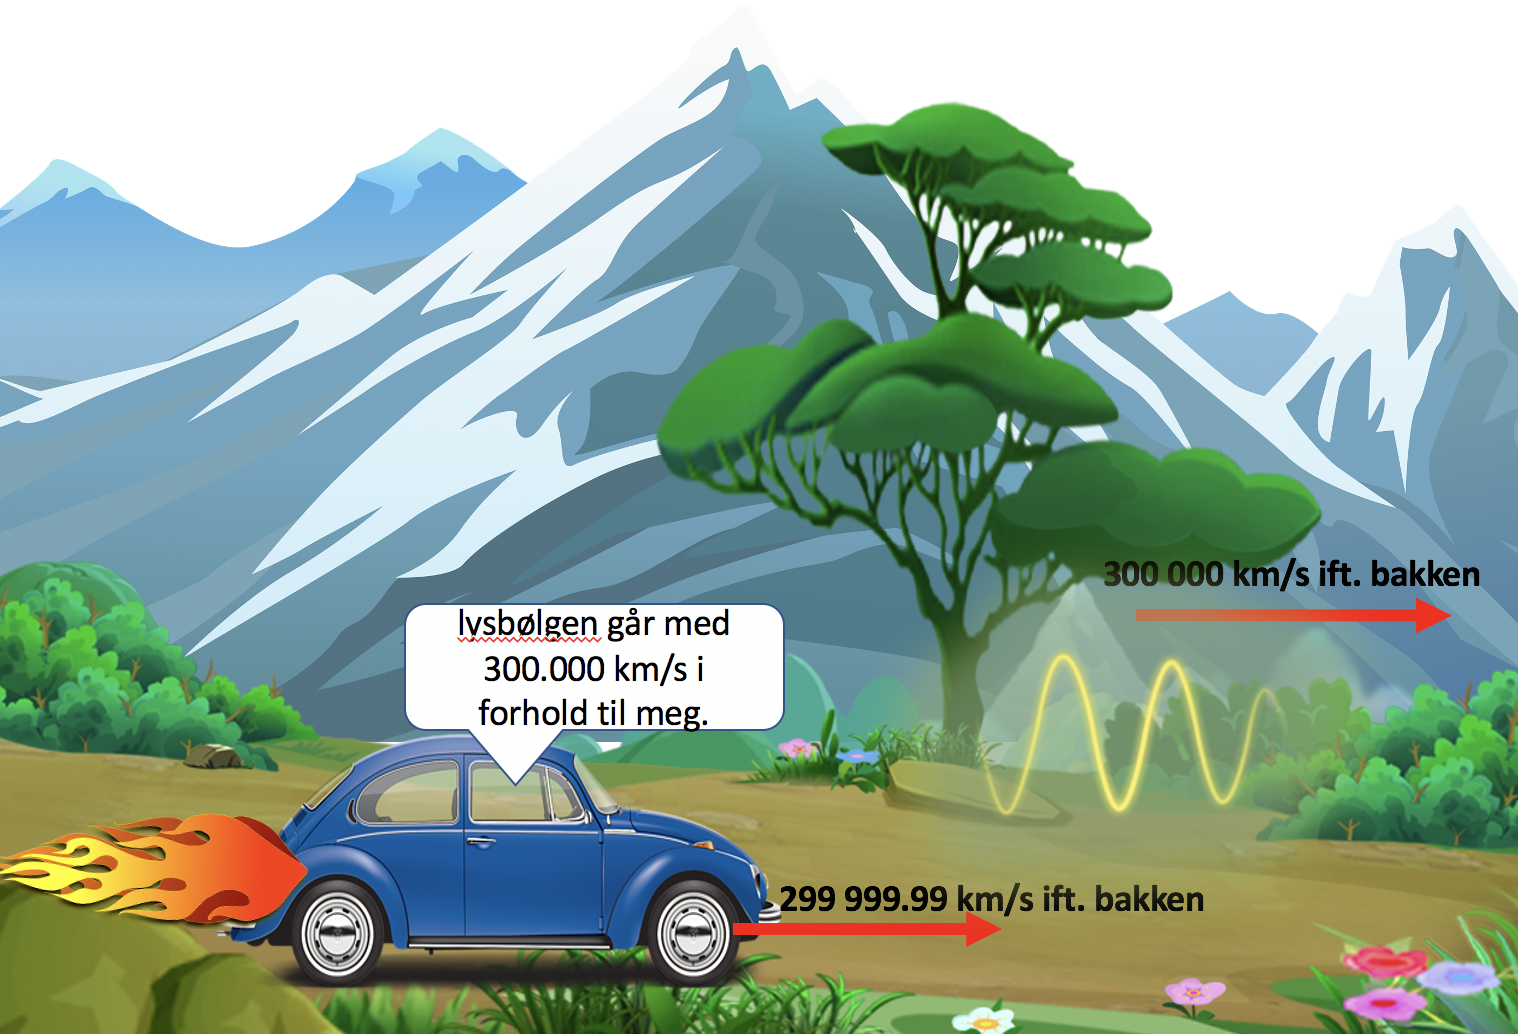
\includegraphics[scale=0.27]{media/klassrel11.png}}
Hvis vi nå bruker sammenhengen
\[
v'_x=\frac{v_x-v_\mathrm{rel}}{1-v_\mathrm{rel}v_x}
\]
hva finner vi? Fra bakken måler vi lyset til å ha lyshastighet $v_x=1$. Hvilken hastighet $v_x'$ vil observatøren i bilen måle at lysstrålen har? Hvordan avhenger det av $v_\mathrm{rel}$?
}{SIDE 30/33/56}

\fullframetxt{hast18b}{hast18}{hast19}{0}{\small Neste side}{\small
La oss gå tilbake til eksemplet i del 2A:
\centerline{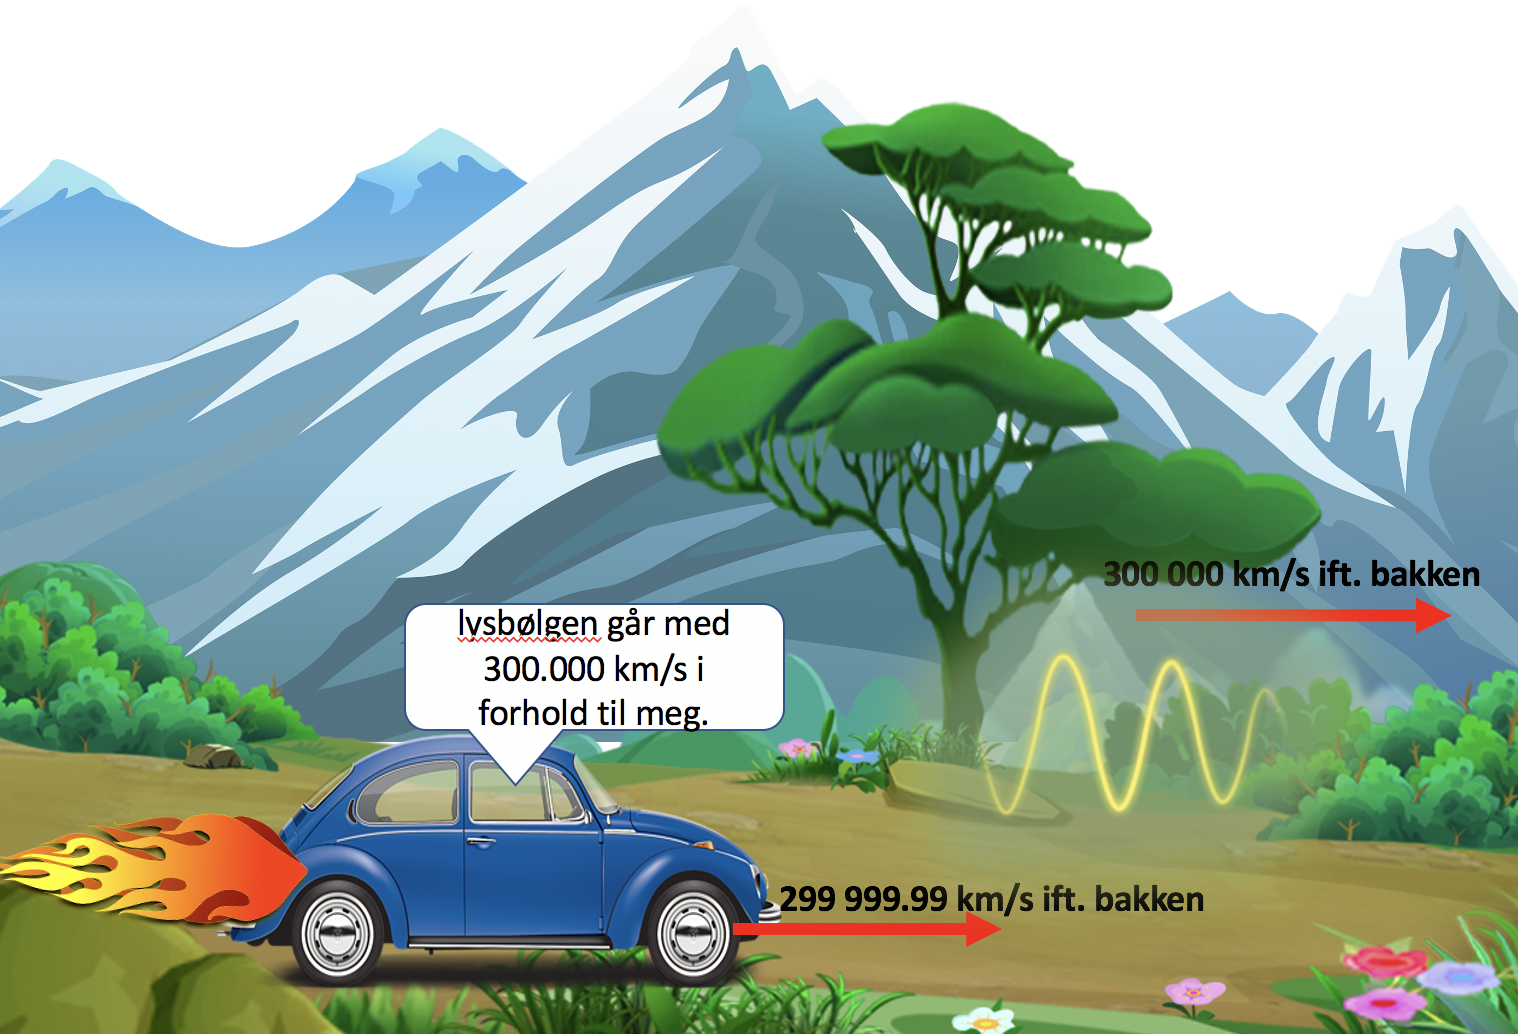
\includegraphics[scale=0.27]{media/klassrel11.png}}
Fikk du ved å sette inn $v_x=1$ her
\[
v'_x=\frac{v_x-v_\mathrm{rel}}{1-v_\mathrm{rel}v_x}
\]
at $v_x'=1$ uansett hva $v_\mathrm{rel}$ er? Det skulle du få!
}{SIDE 31/33/56}



\fullframetxt{hast19}{hast18b}{hast20}{0}{\small Neste side}{\small
\centerline{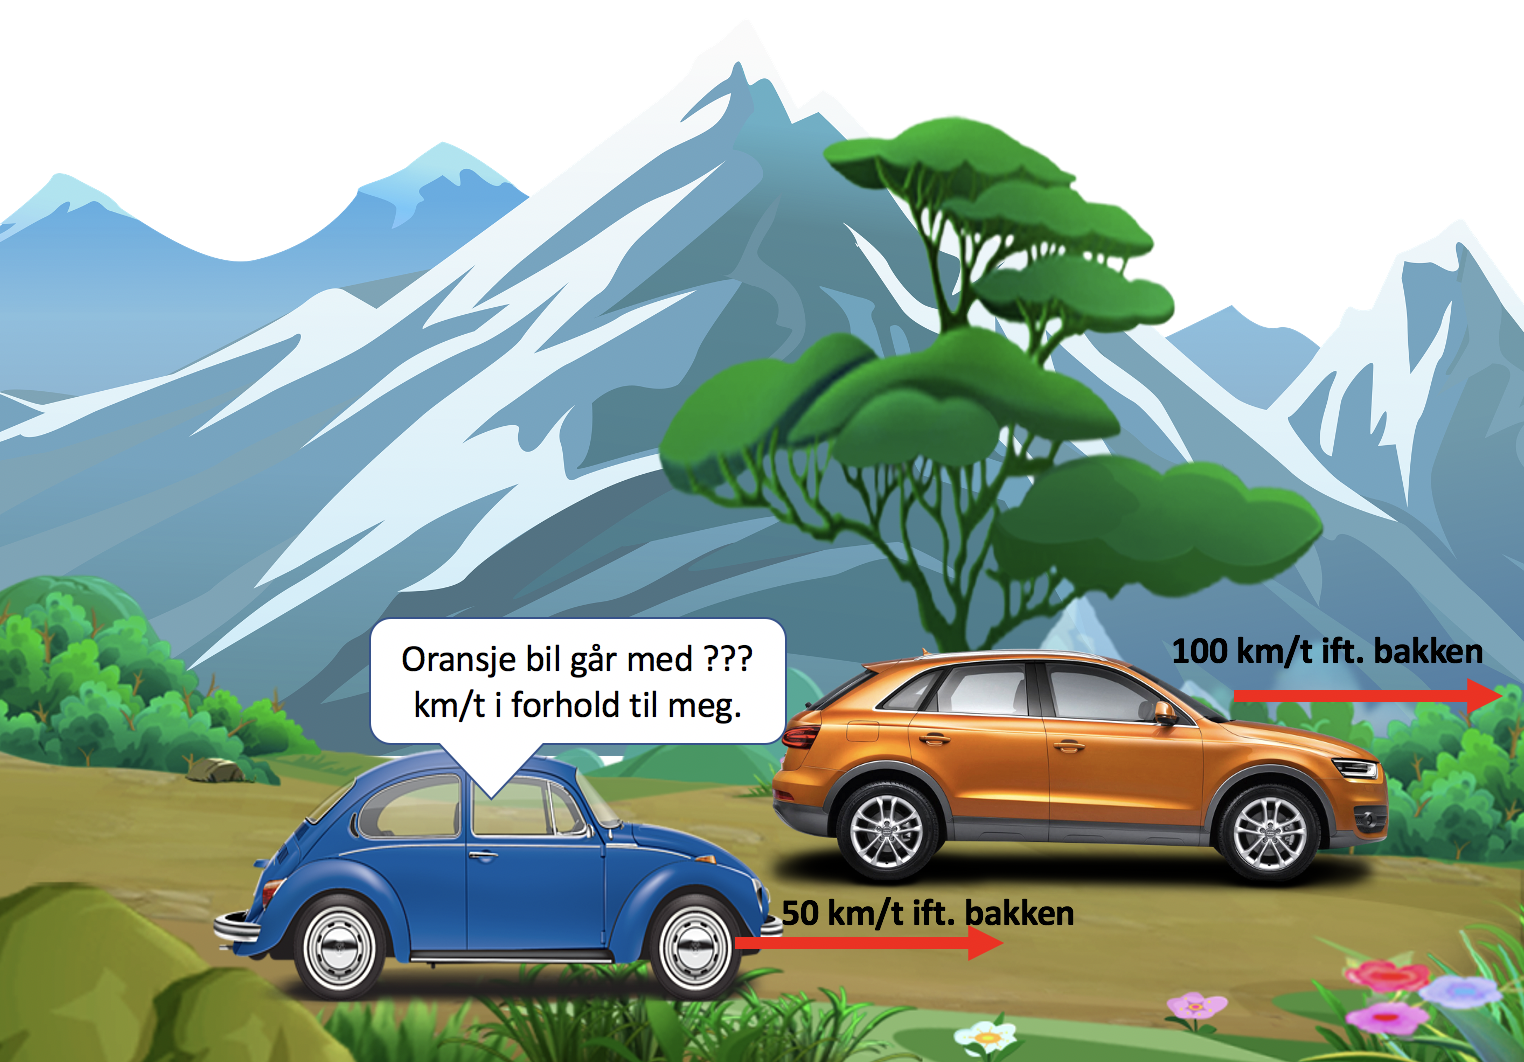
\includegraphics[scale=0.27]{media/klassrel2.png}}
{\bf La oss gå tilbake til eksempler med små hastigheter (se figur):} Hvis vi nå bruker sammenhengen
\[
v'_x=\frac{v_x-v_\mathrm{rel}}{1-v_\mathrm{rel}v_x}
\]
hva finner vi? Her er den relative hastigheten mellom observatørene veldig mye mindre enn lyshastigheten, enig? Vi har at $v_\mathrm{rel}\ll1$. Det samme gjelder $v_x$, hastigheten målt fra bakken. Hva skjer med denne likningen da??? Ikke bla om før du har uttrykket!
}{SIDE 32/33/56}

\fullframetxt{hast20}{hast19}{blue_nytema3}{0}{\footnotesize Neste side}{\footnotesize
\centerline{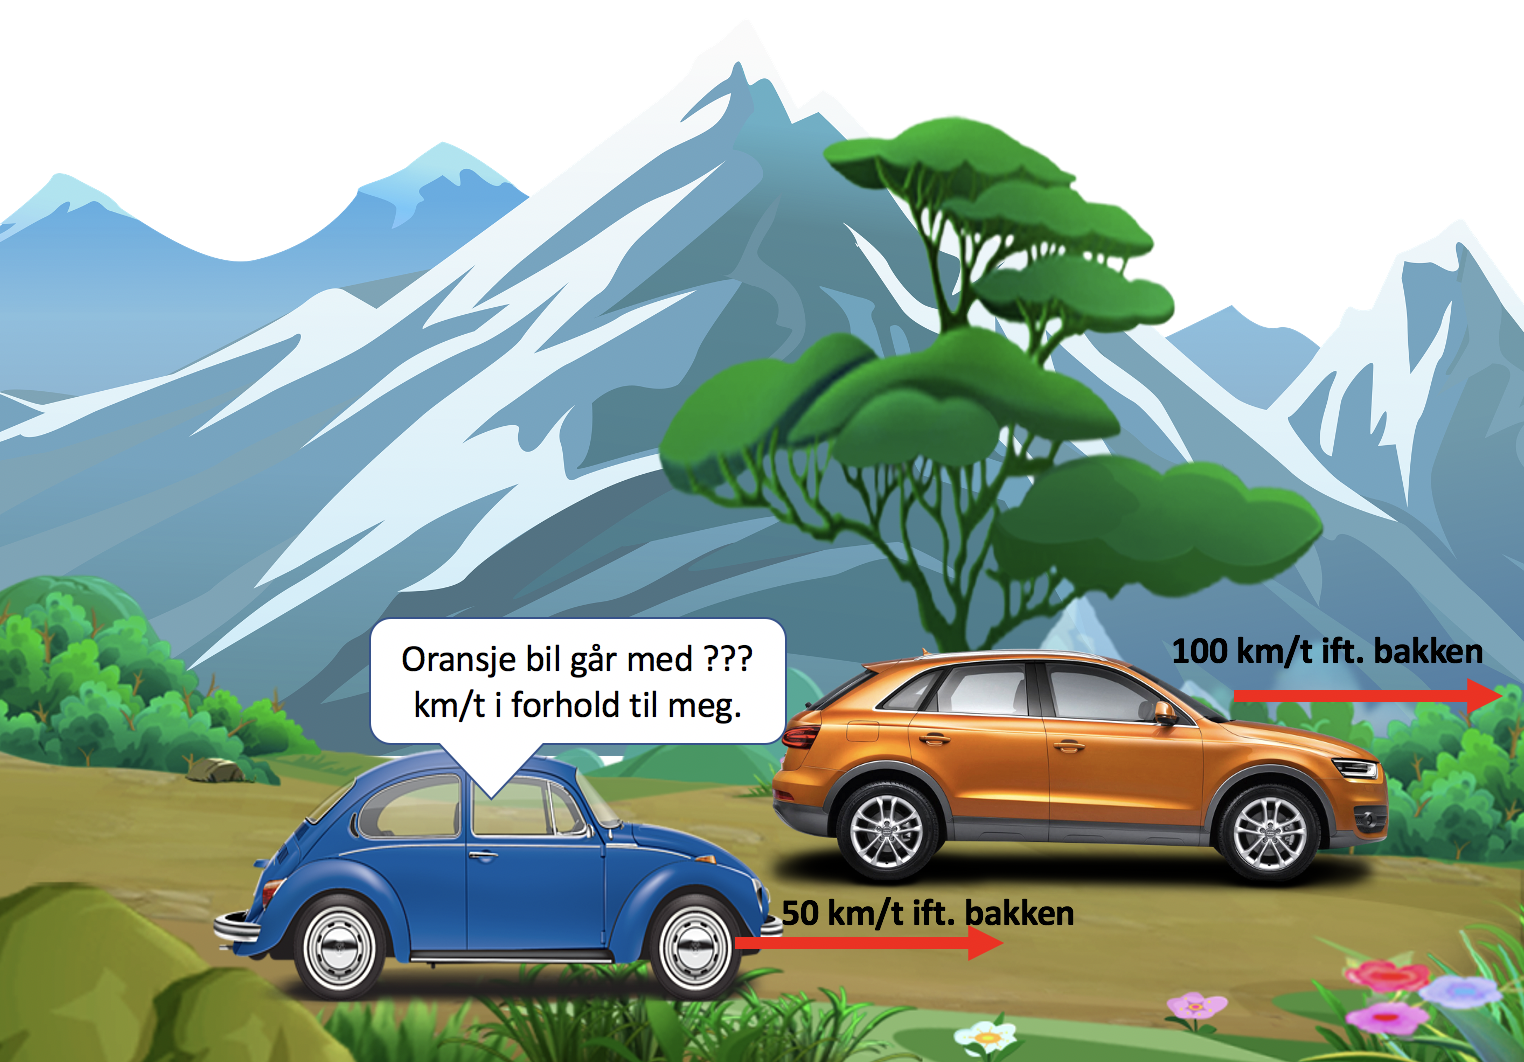
\includegraphics[scale=0.25]{media/klassrel2.png}}
Får du at
\[
v'_x=\frac{v_x-v_\mathrm{rel}}{1-v_\mathrm{rel}v_x}
\]
blir til
\[
v'_x=v_x-v_\mathrm{rel}
\]
når både $v_x$ og $v_\mathrm{rel}$ er mye mindre enn lyshastigheten? {\bf Er ikke dette uttrykket for hastighetstransformasjon i den klassiske relativitetsteorien som vi snakket om i 2A?} (hvis du lurer på hvorfor $v_\mathrm{rel}v_x$ forsvinner her og ikke $v_\mathrm{rel}$ så tenk på hvilke av disse uttrykkene som er minst her? Ta et eksempel med begge hastigheter av størrelseorden f.eks. $10^{-6}$)
}{SIDE 33/33/56}

\renewcommand{\headline}{\small Relativistisk bevegelsesmengde}
{
\setbeamercolor{background canvas}{bg=blue}
\begin{frame}
\label{blue_nytema3}
\hyperlink{hast20}{\pagebutton{\small Forrige side}}
\nytemaside{0}
\textcolor{yellow}{\Large Er du sikker på at du er opplagt til resten av denne forelesningen idag? Kunne du kanskje ta resten imorgen og få klarnet tankene litt?}\\
{\bf\large Det blir en pause underveis...}
\hyperlink{pe1}{\pagebutton{Jeg er klar...}}
\end{frame}
}

\fullframetxt{pe1}{hast20}{pe2}{0}{\label{pm}\footnotesize Neste side}{\footnotesize
{\bf La oss holde oss til dette eksemplet litt til:}\\
\centerline{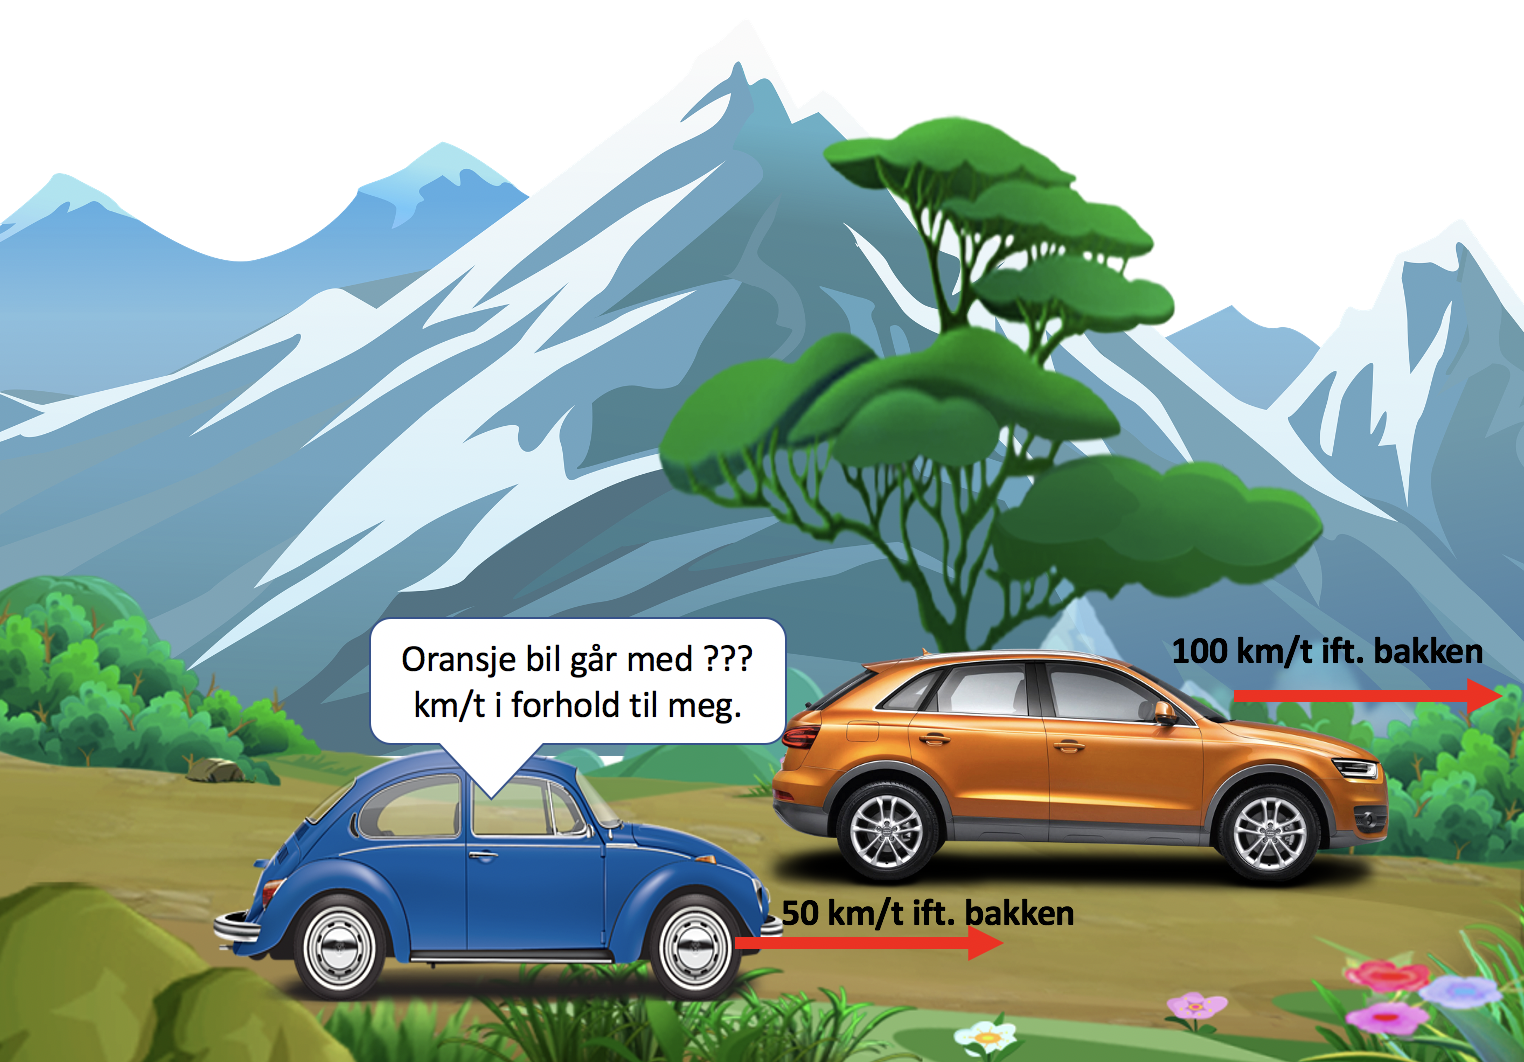
\includegraphics[scale=0.25]{media/klassrel2.png}}
Vi er enige om at bakkeobservatøren og observatøren i den blå bilen måler forskjellige hastigheter for den oransje bilen. Men hvis de måler forskjellige hastigheter, så er de vel heller ikke enige om bevegelsesmengden til oransje bil? Den avhenger jo av hastigheten? Kan vi lage oss en 4-dimensjonal bevegelsesmengde-4-vektor også? {\bf Isåfall hvordan?} Hvordan ville du definert denne?
}{SIDE 34/56/56}

\fullframetxt{pe2}{pe1}{pe3}{0}{\footnotesize Neste side}{
\centerline{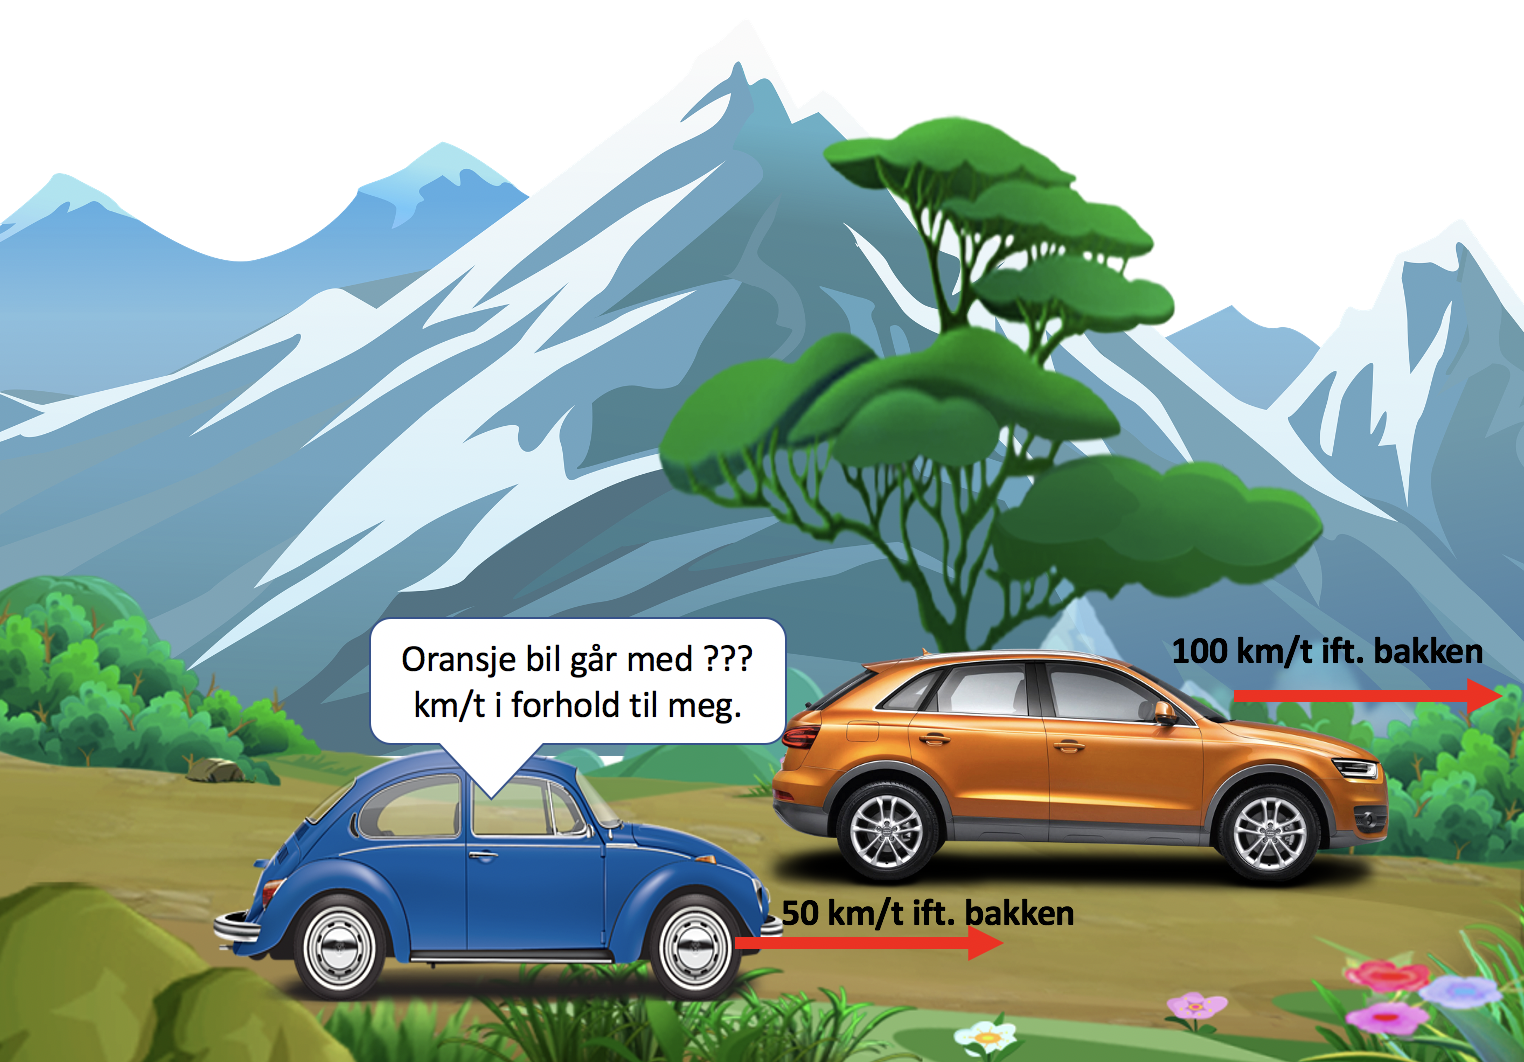
\includegraphics[scale=0.25]{media/klassrel2.png}}
Vi vet at 3-dimensjonal bevegelsesmengde er gitt ved
\[
\vec{p}=m\vec{v}
\]
der $m$ er massen til objektet. Kan vi generalisere dette til 4-dimensjonalt tidrom? Vi har jo allerede 4-dimensjonal hastighet $V_\mu$? Hvordan vil du gjøre dette? Og hva må vi passe på? (lærepengen fra da vi skulle lage oss $V_\mu$)
}{SIDE 35/56/56}


\fullframetxt{pe3}{pe2}{pe4}{0}{\footnotesize Neste side}{
\centerline{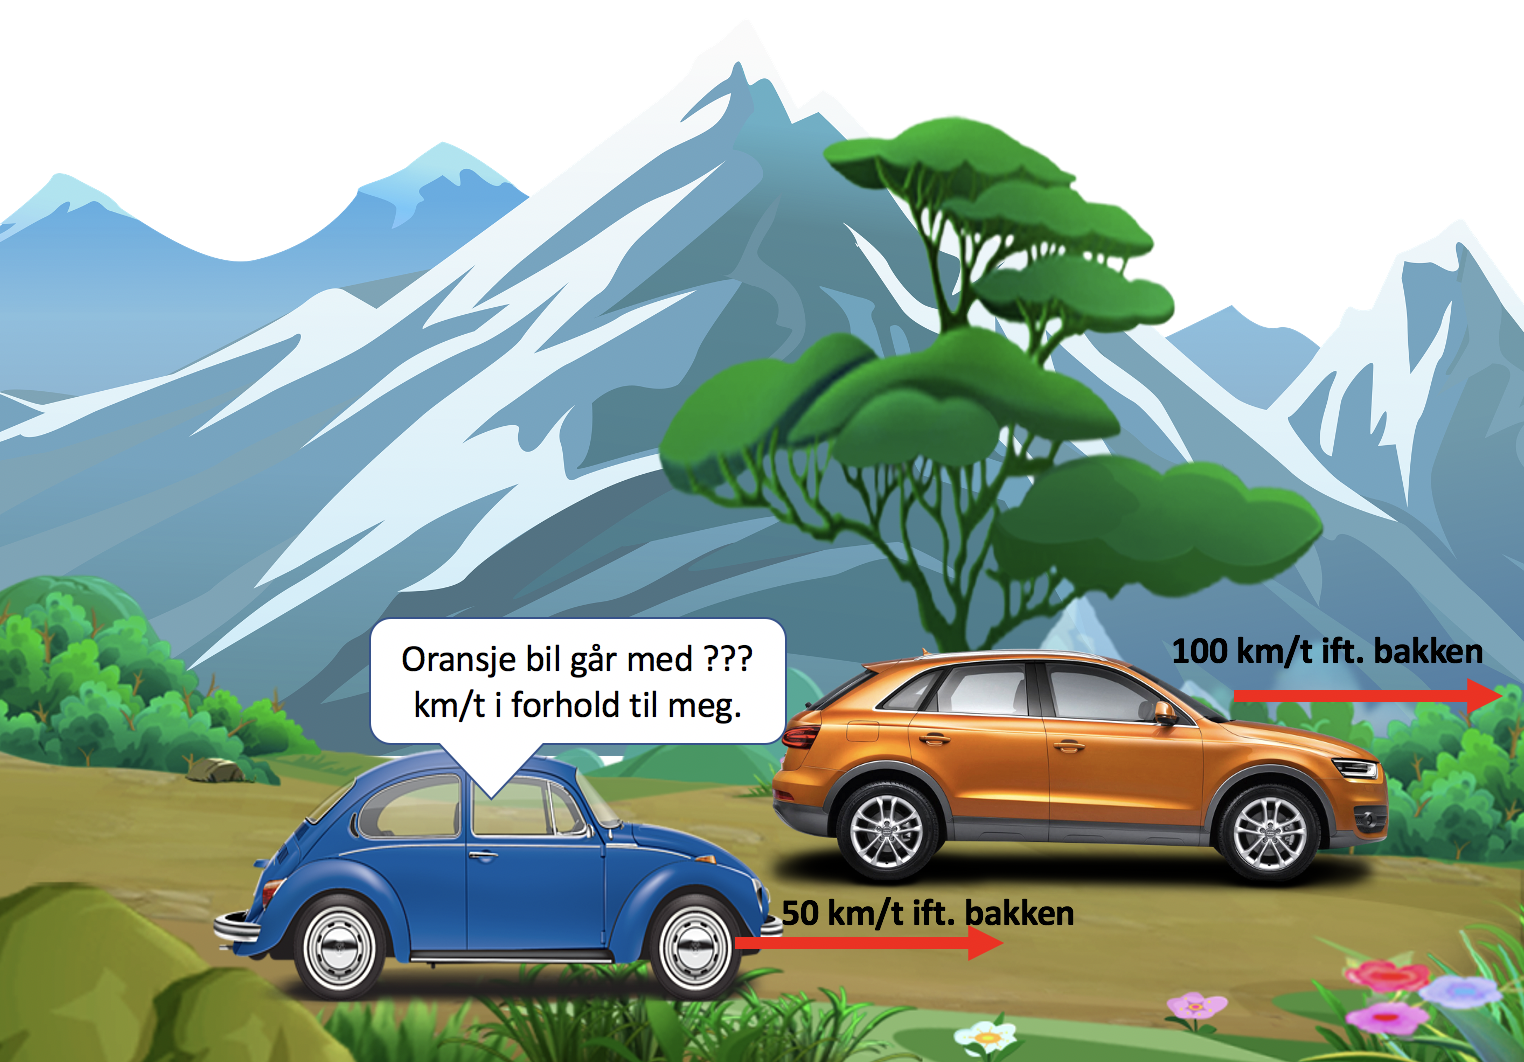
\includegraphics[scale=0.25]{media/klassrel2.png}}
Det er fristende å prøve oss med
\[
P_\mu=mV_\mu
\]
ikke sant? Kan du se noe problem med dette?
}{SIDE 36/56/56}

\fullframetxt{pe4}{pe3}{pe5}{0}{\footnotesize Neste side}{\footnotesize
\[
P_\mu=mV_\mu
\]
Vi må forsikre oss om at massen $m$ er {\bf invariant}, ikke sant? \textcolor{red}{Hvis ikke, så får vi ikke lov til å gange den med en 4-vektor! Men {\bf er} masse en invariant størrelse da?} Vil alle observatører måle den samme massen $m$ for alle objekter? I dette kurset skal vi si \textcolor{red}{\bf JA}. Men hvorfor akkurat i dette kurset? Det er en lang historie som vi ikke skal bruke tid på her, men for å gjøre en lang historie kort: du kan formulere konsistente versjoner av relativitetsteorien der enten
\begin{itemize}
\item {\bf massen er en invariant størrelse} som kun avhenger av partikkelen/legemet/systemet vi ser på, men ikke av hvilket referansesystem denne partikkelen/legemet/systemet er i. {\bf Mens energi $E$ ikke er en invariant størrelse}, {\bf ELLER}
\item {\bf energien er en invariant størrelse men massen ikke er det} (i det siste tilfellet har det mening å snakke om ``hvilemasse'' siden massen da vil avhenge av referansesystem og hvilemasse referer til massen man måler i hvilesystemet) Denne formalismen skal vi {\bf ikke} bruke i dette kurset, og har i stor grad blitt forlatt i moderne fysikk (mens den dessverre henger igjen i mange skolebøker)
\end{itemize}
Vi har altså {\bf definert} masse til å være en invariant størrelse. {\bf På denne måten får man en mer konsistent matematisk formalisme for relativitetsteorien.} (relativitetsteorien åpner altså for å definere enten masse eller energi som invariant, dette er kun et definisjonsspørsmål). {\bf Og når masse da er en invariant størrelse, så gir vår definisjon av 4-bevegelsesmengde over mening!}
}{SIDE 37/56/56}


\fullframetxt{pe5}{pe4}{pe6}{0}{\footnotesize Neste side}{\footnotesize
\centerline{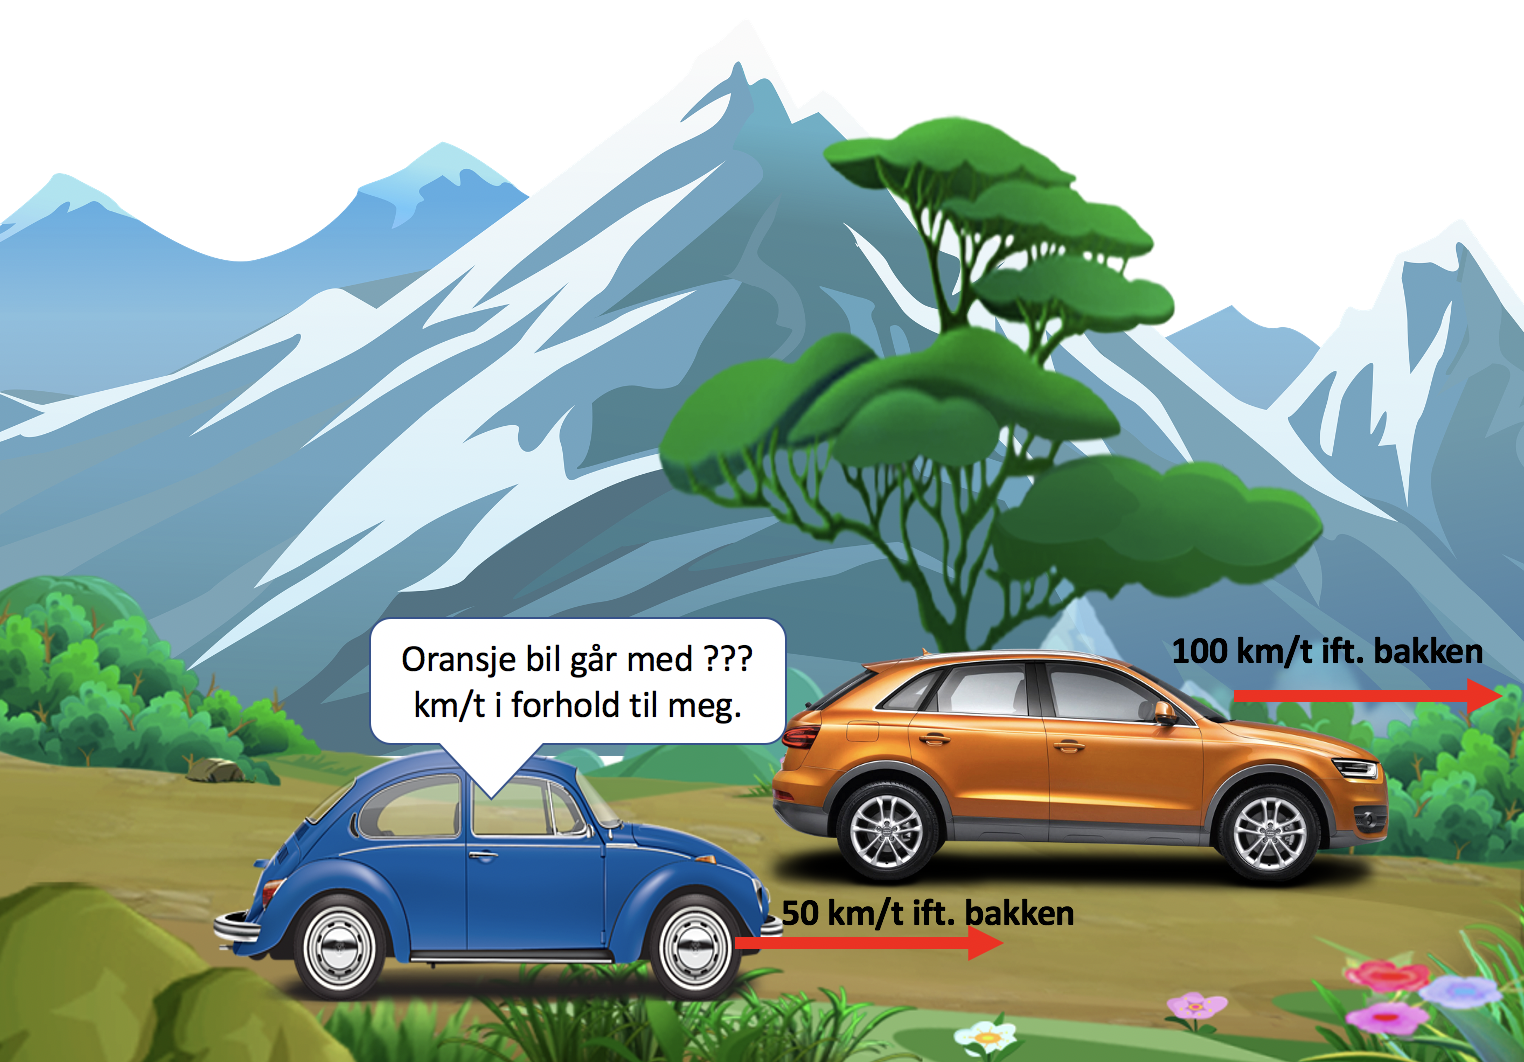
\includegraphics[scale=0.25]{media/klassrel2.png}}
Vi kan altså skrive 4-bevegelsesmengden til den oransje bilen som
\[
P_\mu=mV_\mu=\gamma(m,\vec{p})
\]
der $\vec{p}$ er den vanlige 3D-begelsesmengden målt fra f.eks. bakken. Får du til den siste overgangen her selv? (bruk et uttrykk for $V_\mu$ som vi fant over!).
}{SIDE 38/56/56}

\fullframe{pe6}{pe5}{pe7}{0}{\large
La oss først se på den {\bf romlige} delen av 4-vektoren, altså de 3 siste komponentene av vektoren, den delen av 4-vektoren som tilsvarer posisjon for en posisjons-4-vektor.
\[
P_\mu=mV_\mu=\gamma(m,\vec{p})
\]
Den romlige delen er her $\gamma\vec{p}$. Har du sett dette uttrykket før? Det er uttrykket for relativistisk bevegelsesmengde:
\[
\vec{p}_\mathrm{relativistisk}=\gamma\vec{p}=\gamma m\vec{v}
\]
{\bf Det viser seg i eksperimenter at det er denne relativistiske bevegelsesmengden som er den størrelsen som er bevart!} Den klassiske bevegelsesmengden $\vec{p}=m\vec{v}$ er {\bf ikke} en bevart størrelse slik som du har lært. Men når hastighetene er små, altså $v\ll1$, altså hastigheter mye mindre enn lyshastigheten, så er $\gamma\rightarrow1$ og de to uttrykkene blir like. Men for store hastigheter så {\bf må} man bruke relativistisk bevegelsesmengde. Den klassiske er {\bf ikke} en bevart størrelse.
}{SIDE 39/56/56}

\fullframe{pe7}{pe6}{pe8}{0}{\large
  Det ser virkelig ut til at 4-vektorformalismen har noe for seg! Når vi konstruerer en bevegelsesmengde-4-vektor, så faller det ut at den romlige delen av denne er en svært viktig fysisk størrelse. Det er dette som er det riktige og generelle uttrykket for bevegelsesmengde mens det viser seg at det klassiske uttrykket $\vec{p}=m\vec{v}$ bare er en tilnærmelse for lave hastigheter. 4-vektor-formalismen og det å jobbe med matematiske størrelser i det 4-dimensjonale tidrom ser dermed ut til å kanskje være nærmere slik naturen faktisk funker. Det virker som om vi får resultater som stemmer bedre med virkeligeheten når vi jobber i dette rommet.
}{SIDE 40/56/56}


\fullframetxt{pe8}{pe7}{pause2}{0}{\small Jeg har sett videoen og har fortsatt ikke kommet meg over sjokket!}{\large
La oss se en gang til på 4-bevegelsesmengden:
\[
P_\mu=mV_\mu=\gamma(m,\vec{p})
\]
Kan vi finne en tolkning av {\bf tidsdelen} av denne 4-vektoren? \textcolor{red}{Altså den første komponenten som tilsvarer tid når vi snakker om posisjons-4-vektorer?} Vi ser at den er $\gamma m$. I \href{https://www.uio.no/studier/emner/matnat/astro/AST2000/h20/undervisningsmateriell/interaktive-forelesningsnotater/2b/videoer/video2b_21.mp4}{denne videoen} skal vi ser på hvordan denne størrelsen ser ut i den klassiske grensen, dvs. ved lave hastigheter. Og vi skal gjøre en {\bf stor} og viktig oppdagelse!
}{SIDE 41/56/56}

{
\setbeamercolor{background canvas}{bg=cyan}
\begin{frame}
\label{pause2}
\hyperlink{pe8}{\pagebutton{\small Forrige side}}
\centerline{{\small Kaffe!} Kaffe! {\Large Kaffe} {\huge Kaffe!} {\bf\Huge Kaffe!}}
{\huge
\centerline{
\includegraphics[scale=4]{media/drink-coffee.png}}
Jada, jada, helt klart velfortjent nå! Det verste er overstått, nå er det bare småplukk igjen (viktig småplukk vel og merke!), og så litt spennende saker som er utenfor pensum for de interesserte på de siste sidene...
}\\
\vspace*{0.5cm}
\hyperlink{pe9}{\pagebutton{Jeg er klar til å fortsette...}}
\end{frame}
}

\fullframe{pe9}{pe8}{pe10}{0}{\large
Vi har altså sett at 4-bevegelsesmengdevektoren kan skrives som
\[
P_\mu=(E_\mathrm{relativistisk},\vec{p}_\mathrm{relativistisk})
\]
der
\[
E_\mathrm{relativistisk}=m\gamma
\]
og er en {\bf bevart størrelse} som inneholder både hvileenergien til legemet og den kinetiske i en og samme størrelse. Disse to størrelsene smelter her sammen til en energi. Det er kun ved lave hastigheter at vi ser at dette separeres ut i to forskjellige typer energier. {\bf MERK altså igjen, den klassiske kinetiske energien er ikke en bevart størrelse, men er tilnærmet bevart ved lave hastigheter. Det er kun den relativistiske energien som er en et mer generelt uttrykk for energi og som viser seg å være bevart i eksperimenter!}. \textcolor{red}{Det viser seg altså fra eksperimenter at bevegelsesmengde-4-vektoren $P_\mu$er en bevart størrelse!}
}{SIDE 42/56/56}

\fullframe{pe10}{pe9}{pe11}{0}{\large
Men hva er {\bf lengden} av $P_\mu$ da? Når vi tar lengden av 4-hastigheten $V_\mu$ så fant vi at vi alle har fart lik lyshastigheten. Hva nå med lengden av bevegelsesmengde-4-vektoren? Husker du hvordan vi regnet ut lengde av $V_\mu$? Prøv deg selv nå, se om du kan finne at
\[
P=\sqrt{P_\mu P^\mu}=m
\]
Skalarproduktet gir oss igjen en skalar, nemlig massen til et objekt. Det er den som er lengden av vektoren, og den er konstant. For at lengden av vektoren skal bevares (altså massen bevares) når hastigheten endres (som betyr at bevegelsesmengde og energi endres, disse avhenger begge av hastighet!), må det finnes en relasjon mellom masse, energi og bevegelsesmengde.
}{SIDE 43/56/56}

\fullframe{pe11}{pe10}{pe12x}{0}{\large
Den skal vi finne nå. Ta utgangspunkt i
\[
P_\mu=(E_\mathrm{relativistisk},\vec{p}_\mathrm{relativistisk})
\]
Skriv skalaproduktet ut en gang til, nå uttrykkt ved relativistisk energi og bevegelsesmengde. Sette denne lik det du fant på forrige side. Klarer du å komme frem til...
\begin{block}{...en svært viktig relasjon mellom relativistiske størrelser...}
\[
E_\mathrm{relativistisk}^2-p_\mathrm{relativistisk}^2=m^2
\]
som gjør at du f.eks. hvis du kjenner to av disse størrelsene, kan finne den 3.
\end{block}
{\bf Merk deg denne relasjonen da den ofte er løsningen på problemer der det virker som om informasjon mangler!!!}
}{SIDE 44/56/56}

\fullframe{pe12x}{pe11}{pe12}{0}{\large
Denne relasjonen,
\[
E_\mathrm{relativistisk}^2-p_\mathrm{relativistisk}^2=m^2
\]
gjør også at masseløsepartikler som fotoner faktisk har en bevegelsesmengde. Sett inn $m=0$ og du får
\[
E_\mathrm{relativistisk}^2=p_\mathrm{relativistisk}^2
\]
for fotoner. Vi husker at $E=h\nu$ for fotoner. Dette blir ifølge denne formelen da også størrelsen på fotones bevevegelsesmengde, men {\bf merk} at bevegelsesmengde har en retning og et fortegn mens energi bare er en størrelse. Bevegelsesmengde-4-vektoren for et foton som beveger seg i negativ retning langs x-aksen vil da kunne skrives som:
\[
P_\mu=(E_\mathrm{relativistisk},\vec{p}_\mathrm{relativistisk})=(h\nu,-h\nu,0,0)
\]
}{SIDE 45/56/56}

\fullframenotxt{pe12}{pe12x}{pe13}{0}{\small
La du merke til noe rart i dette uttrykket?
\[
E_\mathrm{relativistisk}^2-p_\mathrm{relativistisk}^2=m^2
\]
\hyperlink{pe12_b}{\pagebutton{Tjaaaaaaa...}}\\
\textcolor{white}{
Hva med enhetene i denne likningen da?\\
{Dæggern... her varre no'rart...}\\
Sa jo det jo! Men egentlig ikke så rart. Vi bruker jo nå konsekvent at vi har samme enheter for tidsintervaller som for romlige avstander. Dette endrer også andre enheter. Det gjør at vi nå {\bf måler både masse, bevegelsesmengde og energi i kg!}. Dette faller automatisk ut av at vi bruker like enheter på tid og rom. For å gjøre om til vanlige SI enheter trenger du da å gjøre
\begin{align*}
E(\mathrm{Joule})&=E(\mathrm{kg})c^2\\
p(\mathrm{kg\,m/s})&=p(\mathrm{kg})c
\end{align*}
Det er naturligvis lyshastigheten som kommer inn i omregningen siden det var den vi brukte for å regne om meter til sekunder og omvendt.}
}{SIDE 46/56/56}

\fullframenotxt{pe12_b}{pe12x}{pe13}{0}{\small
La du merke til noe rart i dette uttrykket?
\[
E_\mathrm{relativistisk}^2-p_\mathrm{relativistisk}^2=m^2
\]
{\pagebutton{Tjaaaaaaa...}}\\
Hva med enhetene i denne likningen da?\\
\hyperlink{pe12_c}{\pagebutton{Dæggern... her varre no'rart...}}\\
\textcolor{white}{
Sa jo det jo! Men egentlig ikke så rart. Vi bruker jo nå konsekvent at vi har samme enheter for tidsintervaller som for romlige avstander. Dette endrer også andre enheter. Det gjør at vi nå {\bf måler både masse, bevegelsesmengde og energi i kg!}. Dette faller automatisk ut av at vi bruker like enheter på tid og rom. For å gjøre om til vanlige SI enheter trenger du da å gjøre
\begin{align*}
E(\mathrm{Joule})&=E(\mathrm{kg})c^2\\
p(\mathrm{kg\,m/s})&=p(\mathrm{kg})c
\end{align*}
Det er naturligvis lyshastigheten som kommer inn i omregningen siden det var den vi brukte for å regne om meter til sekunder og omvendt.}
}{SIDE 46/56/56}

\fullframe{pe12_c}{pe12x}{pe13}{0}{\small
La du merke til noe rart i dette uttrykket?
\[
E_\mathrm{relativistisk}^2-p_\mathrm{relativistisk}^2=m^2
\]
{\pagebutton{Tjaaaaaaa...}}\\
Hva med enhetene i denne likningen da?\\
{\pagebutton{Dæggern... her varre no'rart...}}\\
Sa jo det jo! Men egentlig ikke så rart. Vi bruker jo nå konsekvent at vi har samme enheter for tidsintervaller som for romlige avstander. Dette endrer også andre enheter. Det gjør at vi nå {\bf måler både masse, bevegelsesmengde og energi i kg!}. Dette faller automatisk ut av at vi bruker like enheter på tid og rom. For å gjøre om til vanlige SI enheter trenger du da å gjøre
\begin{align*}
E(\mathrm{Joule})&=E(\mathrm{kg})c^2\\
p(\mathrm{kg\,m/s})&=p(\mathrm{kg})c
\end{align*}
Det er naturligvis lyshastigheten som kommer inn i omregningen siden det var den vi brukte for å regne om meter til sekunder og omvendt.
}{SIDE 46/56/56}








\fullframetxt{pe13}{pe12}{pe14}{1}{\footnotesize Neste side}{\footnotesize
La oss igjen gå tilbake til eksemplet i del 2A:
\centerline{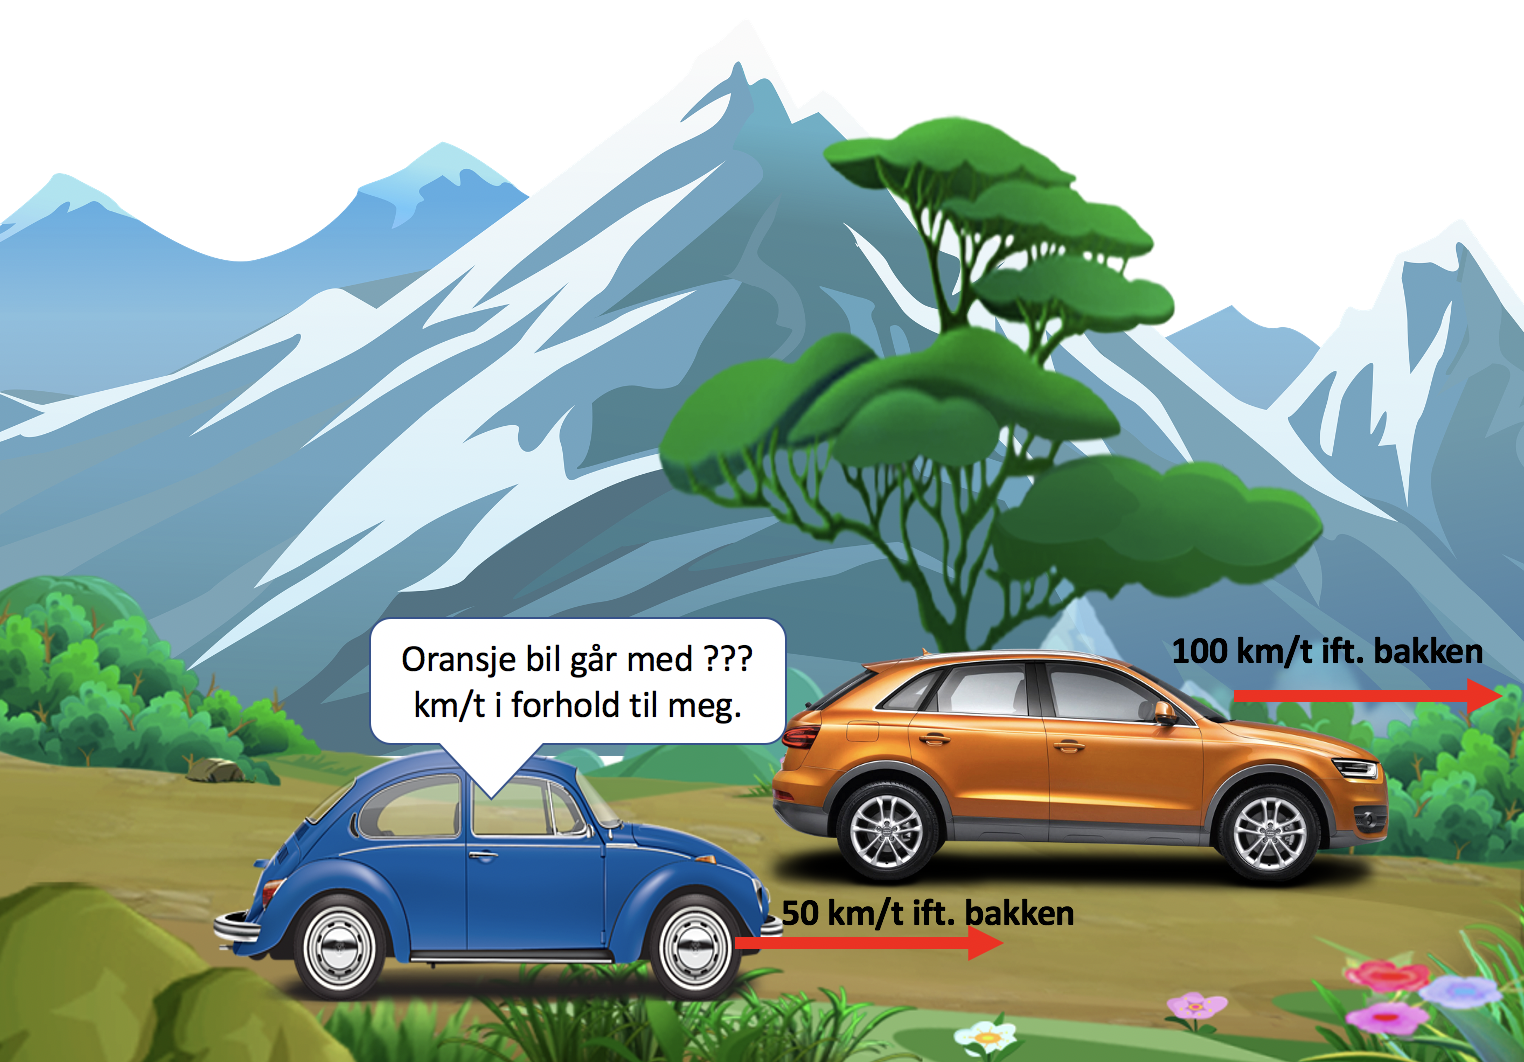
\includegraphics[scale=0.22]{media/klassrel2.png}}
Den oransje bilen har bevegelsesmengde og energi (fra bakkesystemet)
\[
p_x(\mathrm{relativistisk})=\gamma mv_x\ \ \ \ \ E_\mathrm{relativistisk}=\gamma m
\]
der $p_x$ og $v_x$ er bevegelsesmengde og hastighet på den oransje bilen målt fra bakken og $m$ er bilens masse. Målt fra den blå bilen derimot, har den oransje bilen bevegelsesmengde og energi
\[
p_x'(\mathrm{relativistisk})=\gamma' mv_x'\ \ \ \ \ E_\mathrm{relativistisk}=\gamma' m
\]
der
\[
\gamma'=\frac{1}{1-(v_x')^2}
\]
}{SIDE 47/56/56}

\fullframetxt{pe14}{pe13}{red_pe15}{0}{Dette har jeg gjort før, så det kan jeg!}{
\centerline{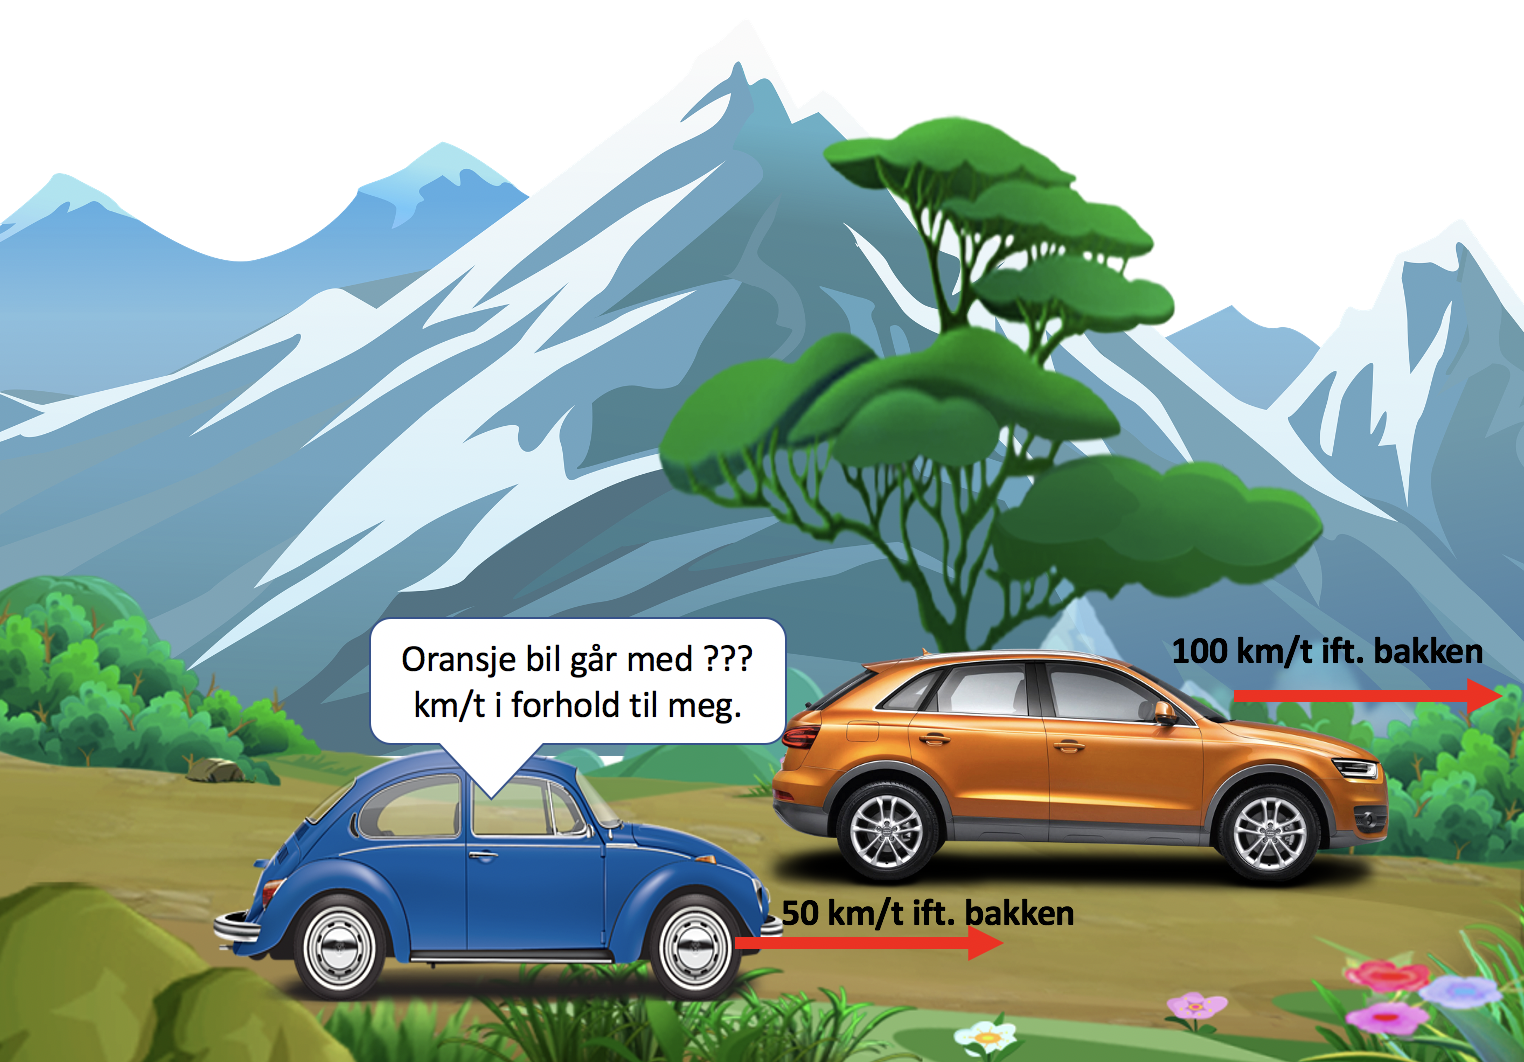
\includegraphics[scale=0.22]{media/klassrel2.png}}
{\bf Men sett at du kun kjenner bevegelsesmengden og energien i det umerkede systemet og ønsker å finne de i det merkede systemet? Du måler $\vec{p}_\mathrm{relativistisk}$ og $E_\mathrm{relativistisk}$ for den oransje bilen fra bakken, men ønsker å vite hva observatøren i den blå bilen måler for disse størrelsene?} Og du kjenner den relative hastigheten $v_\mathrm{rel}$ mellom de to observaørene! Hvordan kan du nå gå frem?
}{SIDE 48/56/56}

\colfullframe{red_pe15}{pe14}{pe16}{0}{red}{\Huge
\textcolor{yellow}{Ja, nå bør du begynne å lukte lunta når du blir spurt om å transformere en størrelse fra et referansesystem til et annet! Da bør du prøve å finne en passende 4-vektor, og bruke de kjente transformasjonsegenskapene til en 4-vektor. Hva er disse?}
}{SIDE 49/56/56}


\fullframe{pe16}{red_pe15}{pe17}{0}{
\centerline{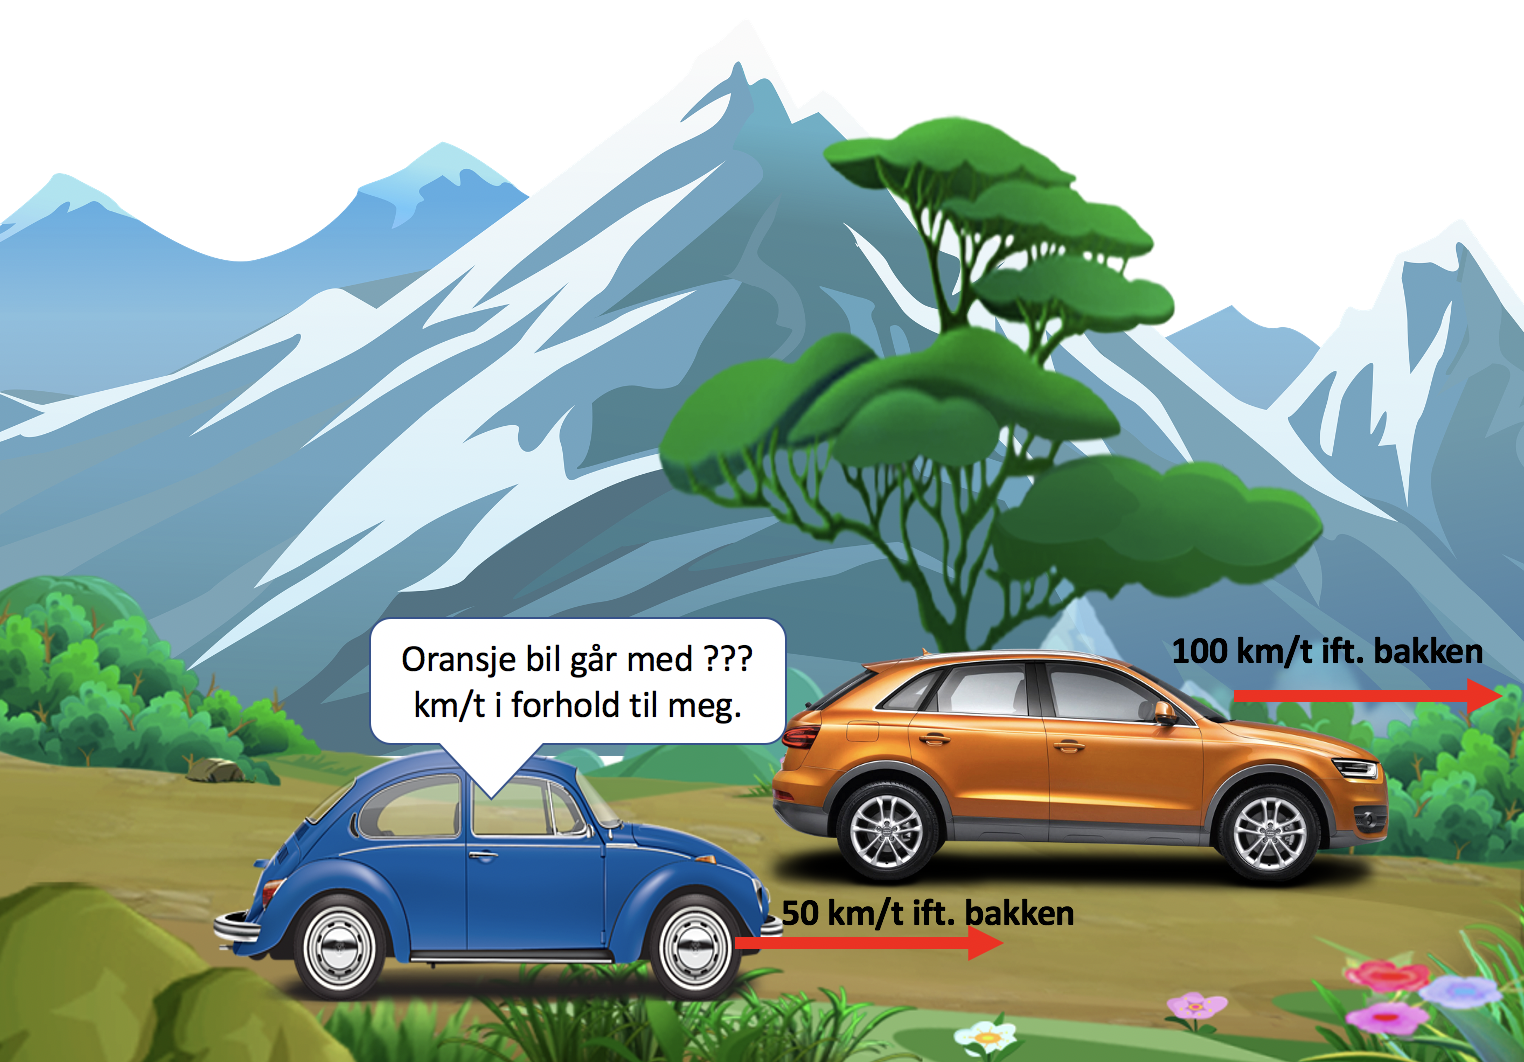
\includegraphics[scale=0.22]{media/klassrel2.png}}
Prøv nå å gjøre transformasjonen og se om du kommer frem til:
\begin{align*}
E'&=\gamma_\mathrm{rel}E-v_\mathrm{rel}\gamma_\mathrm{rel}p_x\\
p_x'&=-v_\mathrm{rel}\gamma_\mathrm{rel}E+\gamma_\mathrm{rel}p_x
\end{align*}
der $E$ og $p_x$ er {\bf relativistiske} bevegelsesmengder og energier og
\[
\gamma_\mathrm{rel}=\frac{1}{\sqrt{1-v_\mathrm{rel}^2}}
\]
}{SIDE 50/56/56}

\fullframe{pe17}{pe16}{pe17b0}{0}{\Huge
Fikk du det til? Hvis ikke, se på \href{https://www.uio.no/studier/emner/matnat/astro/AST2000/h20/undervisningsmateriell/interaktive-forelesningsnotater/2b/videoer/video2b_22.mp4}{denne videoen}. Merk at denne typen transformasjoner bør du kunne gjøre!
}{SIDE 51/56/56}


\fullframe{pe17b0}{pe17}{pe17b}{0}{\footnotesize
Til slutt skal vi se på kjernereaksjoner. Anbefaler at du leser forelesningsnotat 3C om kjernereaksjoner før du fortsetter her. Vi sa der at den totale massen til en atomkjerne ikke tilsvarer summen av massene til kjernepartiklene.  Det var dette som gjør at masse per nukleon avhenger av atomkjernen. For eksempel en heliumkjerne består av 2 protoner og 2 nøytroner, men massen av heliumkjernen er {\bf ikke} lik summen av massene til 2 protoner og 2 nøytroner. Vi skal ikke gjøre noen nøyaktige beregninger her, men illustrere prinsippet med et forenklet eksempel. Anta at du har en atomkjerne med to like (uspesifiserte) kjernepartikler med masse $m$:
\centerline{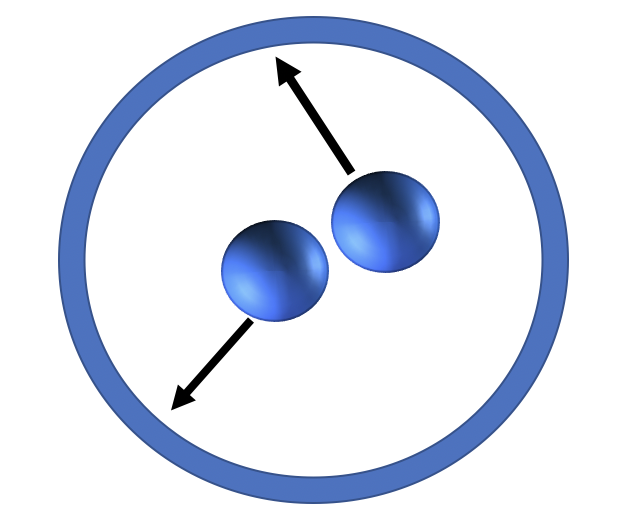
\includegraphics[scale=0.3]{media/nucleus1.png}}\\
Den blå ringen illustrerer atomkjernens størrelse. Kjernepartiklene oppfører seg altså omtrent som gasspartikler med tilfeldige hastigheter som endrer seg hele tiden med holdes innenfor den blå sirkelen av den sterke kjernekrafta.
}{SIDE 52a/56/56}

\fullframenotxt{pe17b}{pe17b0}{pe17c}{0}{\footnotesize
Her skal vi se på et øyeblikksbilde som gjør det lett å regne:
\centerline{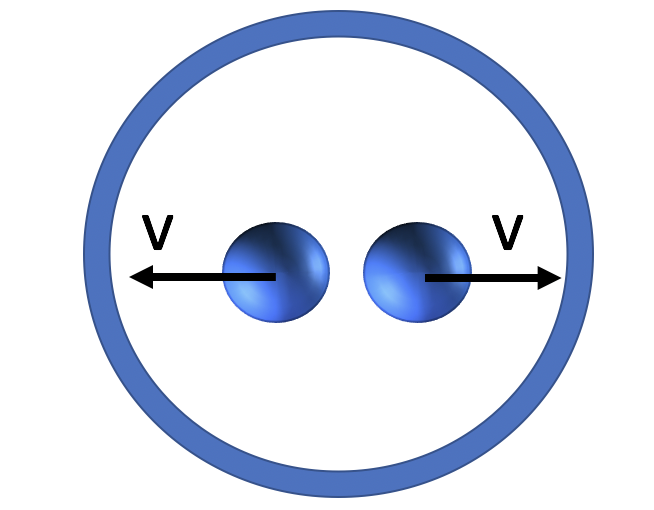
\includegraphics[scale=0.3]{media/nucleus2.png}}\\
Partiklene går her i nøyaktig motsatt regning med samme fart $v$. Etter litt tid vil de selvfølgelig bli dradd tilbake igjen av den sterke kjernekrafta. Sett opp 4-bev.mengdevektoren $P_\mu(1)$ og $P_\mu(2)$ for begge partiklene hver for seg og sum så disse sammen til $P_\mu(M)$ for hele atomkjernen. Du kan uttrykke svaret med massen $m$ og farta $v$. \hyperlink{pe17b_b}{\pagebutton{Ok, har gjort det!}} \textcolor{white}{Fikk du $P_\mu(1)=(\gamma m, \gamma mv)$ og $P_\mu(2)=(\gamma m, -\gamma mv)$??? Og for kjernen $P(M)=(2m\gamma,0)$??}
}{SIDE 52b/56/56}


\fullframe{pe17b_b}{pe17b0}{pe17c}{0}{\footnotesize
Her skal vi se på et øyeblikksbilde som gjør det lett å regne:
\centerline{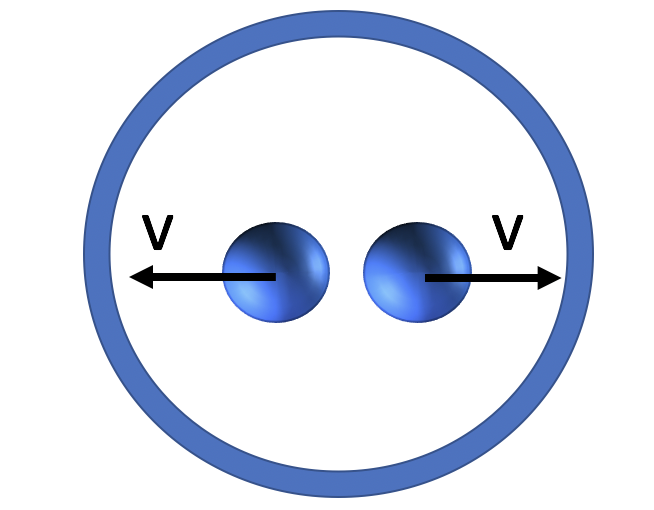
\includegraphics[scale=0.3]{media/nucleus2.png}}\\
Partiklene går her i nøyaktig motsatt regning med samme fart $v$. Etter litt tid vil de selvfølgelig bli dradd tilbake igjen av den sterke kjernekrafta. Sett opp 4-bev.mengdevektoren $P_\mu(1)$ og $P_\mu(2)$ for begge partiklene hver for seg og sum så disse sammen til $P_\mu(M)$ for hele atomkjernen. Du kan uttrykke svaret med massen $m$ og farta $v$. {\pagebutton{Ok, har gjort det!}} Fikk du $P_\mu(1)=(\gamma m, \gamma mv)$ og $P_\mu(2)=(\gamma m, -\gamma mv)$??? Og for kjernen $P(M)=(2m\gamma,0)$??
}{SIDE 52b/56/56}




\fullframetwonotxt{pe17c}{pe17b}{pe18}{1}{
\centerline{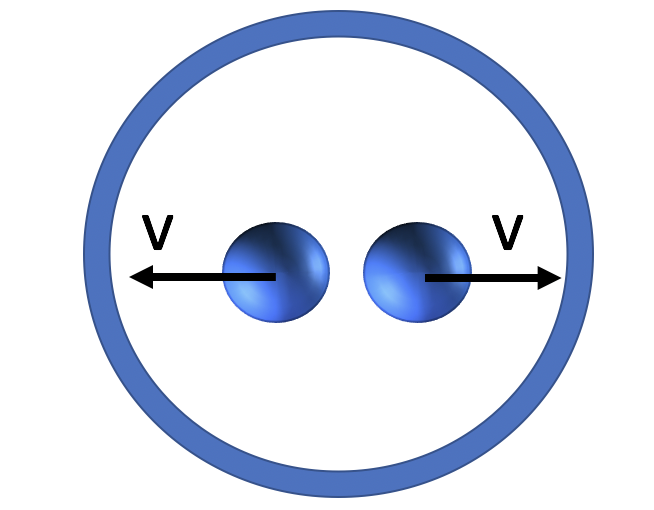
\includegraphics[scale=0.35]{media/nucleus2.png}}
Hvordan finner man massen av en partikkel med 4-bev.mengdevektor $P_\mu$??\hyperlink{pe17c_b}{\pagebutton{\small Det har vi jo akkurat lært...}} \textcolor{white}{Javisst ja, man tar skalarprodukt, $M=\sqrt{P_\mu(M)P^\mu(M)}$. Så hva blir totalmassen til atomkjernen? {\small Regne, regne, regne, det blir...}
\[
M=\sqrt{(2m\gamma)^2-0^2}=2m\gamma
\]}
}
{\textcolor{white}{
{\bf som ikke er $2m$ som vi hadde regnet med hvis masser hadde vært en additiv størrelse!} Merk at atomkjernens totalmasse $2m\gamma$ er en {\bf invariant} størrelse! Alle observatører vil være enige om denne massen siden lengden av $P_\mu$ er en skalar. Vi ser at hastigheten/energien til partiklene inne i atomkjernen bidrar til total masse. Merk også at dette aldri kan skje for en enkelt partikkel, da viste vi for noen sider siden at lengden av $P_\mu$ er partikkelens masse uansett hva dens hastighet er.}
}{SIDE 53/56/56}

\fullframetwonotxt{pe17c_b}{pe17b}{pe18}{1}{
\centerline{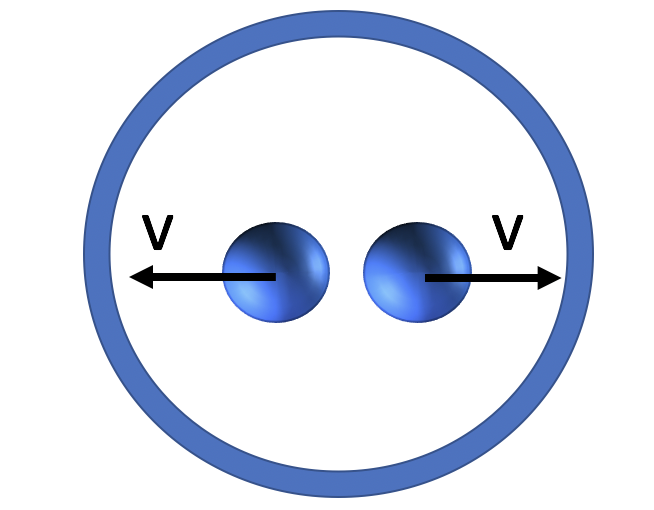
\includegraphics[scale=0.35]{media/nucleus2.png}}
Hvordan finner man massen av en partikkel med 4-bev.mengdevektor $P_\mu$??{\pagebutton{\small Det har vi jo akkurat lært...}} Javisst ja, man tar skalarprodukt, $M=\sqrt{P_\mu(M)P^\mu(M)}$. Så hva blir totalmassen til atomkjernen? \hyperlink{pe17c_c}{\pagebutton{\small Regne, regne, regne, det blir...}}\textcolor{white}{
\[
M=\sqrt{(2m\gamma)^2-0^2}=2m\gamma
\]}
}
{\textcolor{white}{
{\bf som ikke er $2m$ som vi hadde regnet med hvis masser hadde vært en additiv størrelse!} Merk at atomkjernens totalmasse $2m\gamma$ er en {\bf invariant} størrelse! Alle observatører vil være enige om denne massen siden lengden av $P_\mu$ er en skalar. Vi ser at hastigheten/energien til partiklene inne i atomkjernen bidrar til total masse. Merk også at dette aldri kan skje for en enkelt partikkel, da viste vi for noen sider siden at lengden av $P_\mu$ er partikkelens masse uansett hva dens hastighet er.}
}{SIDE 53/56/56}

\fullframetwo{pe17c_c}{pe17b}{pe18}{1}{
\centerline{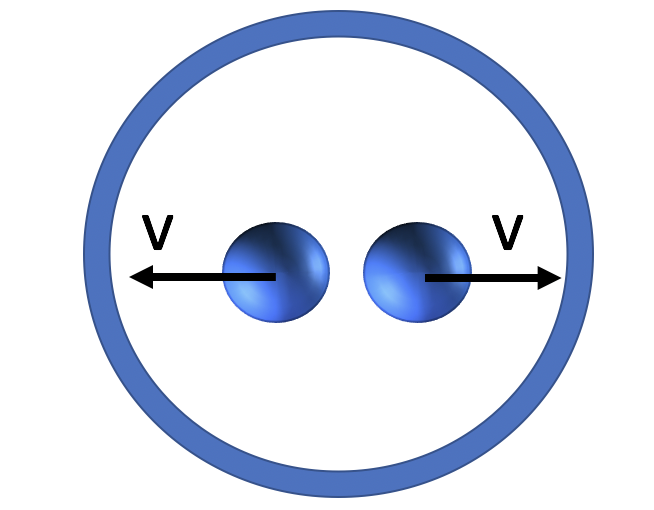
\includegraphics[scale=0.35]{media/nucleus2.png}}
Hvordan finner man massen av en partikkel med 4-bev.mengdevektor $P_\mu$??{\pagebutton{\small Det har vi jo akkurat lært...}} Javisst ja, man tar skalarprodukt, $M=\sqrt{P_\mu(M)P^\mu(M)}$. Så hva blir totalmassen til atomkjernen? {\pagebutton{\small Regne, regne, regne, det blir...}}
\[
M=\sqrt{(2m\gamma)^2-0^2}=2m\gamma
\]
}
{
{\bf som ikke er $2m$ som vi hadde regnet med hvis masser hadde vært en additiv størrelse!} Merk at atomkjernens totalmasse $2m\gamma$ er en {\bf invariant} størrelse! Alle observatører vil være enige om denne massen siden lengden av $P_\mu$ er en skalar. Vi ser at hastigheten/energien til partiklene inne i atomkjernen bidrar til total masse. Merk også at dette aldri kan skje for en enkelt partikkel, da viste vi for noen sider siden at lengden av $P_\mu$ er partikkelens masse uansett hva dens hastighet er.
}{SIDE 53/56/56}







\fullframe{pe18}{pe17c}{pe19}{2}{\huge
\textcolor{red}{Vi skal avslutte med en tur {\bf utenfor pensum}}. For det første, la meg nevne {\bf tensorbegrepet}: Går man videre med 4-vektorformalismen, så innfører man også noe som heter {\bf tensorer}. Dette er en utvidelse av matrisebegrepet til 4-dimensjonalt tidrom, på samme måte som 4-vektorer er en utvidelse av vektorbegrepet til 4-dimensjonalt tidrom.
}{SIDE 54/56/56}


\fullframe{pe19}{pe18}{pe20}{0}{
{\bf Vi avslutter med Maxwells likninger på 4-vektor-formalisme: (\textcolor{red}{Også utenfor pensum!})}\\
{\Huge
\vspace*{-1cm}
\[
\square A^\mu=\mu_0J^\mu
\]
}
{\bf Dette er alle Maxwells likninger, som i 4-vektorformalismen kun blir denne lille likningen!}
Her er
\[
A^\mu=(\phi,\vec{A})
\]
{\bf 4-potensial} der tidskomponenten av 4-vektoren er elektromagnetisk potensial $\phi$ og romkomponenten er magnetisk potensial $\vec{A}$. Vi ser også at vi har
\[
J^\mu=(\rho,\vec{j})
\]
som er {\bf 4-strøm} der tidsdelen er ladning og romdelen er elektrisk strøm. Firkanten $\square$ er d'Alembert-operatoren som tilsvarer nabla $\nabla$ i 4-dimensjonalt tidrom. {\bf Denne ene og korte likningen er ekvivalent med alle 4 Maxwell-likningene}. Vi ser igjen at likninger blir mye mer elegante i 4-dimensjonalt tidrom.
}{SIDE 55/56/56}

\fullframe{pe20}{pe19}{oppsummering}{0}{\small
{\bf Har du lyst til å sove dårlig om natta!} Da kan du ta en kikk på dette ``paradokset'' (det er faktisk {\bf ikke} et paradoks, bare ser slik ut) som \textcolor{red}{\bf også er utenfor pensum:}
\centerline{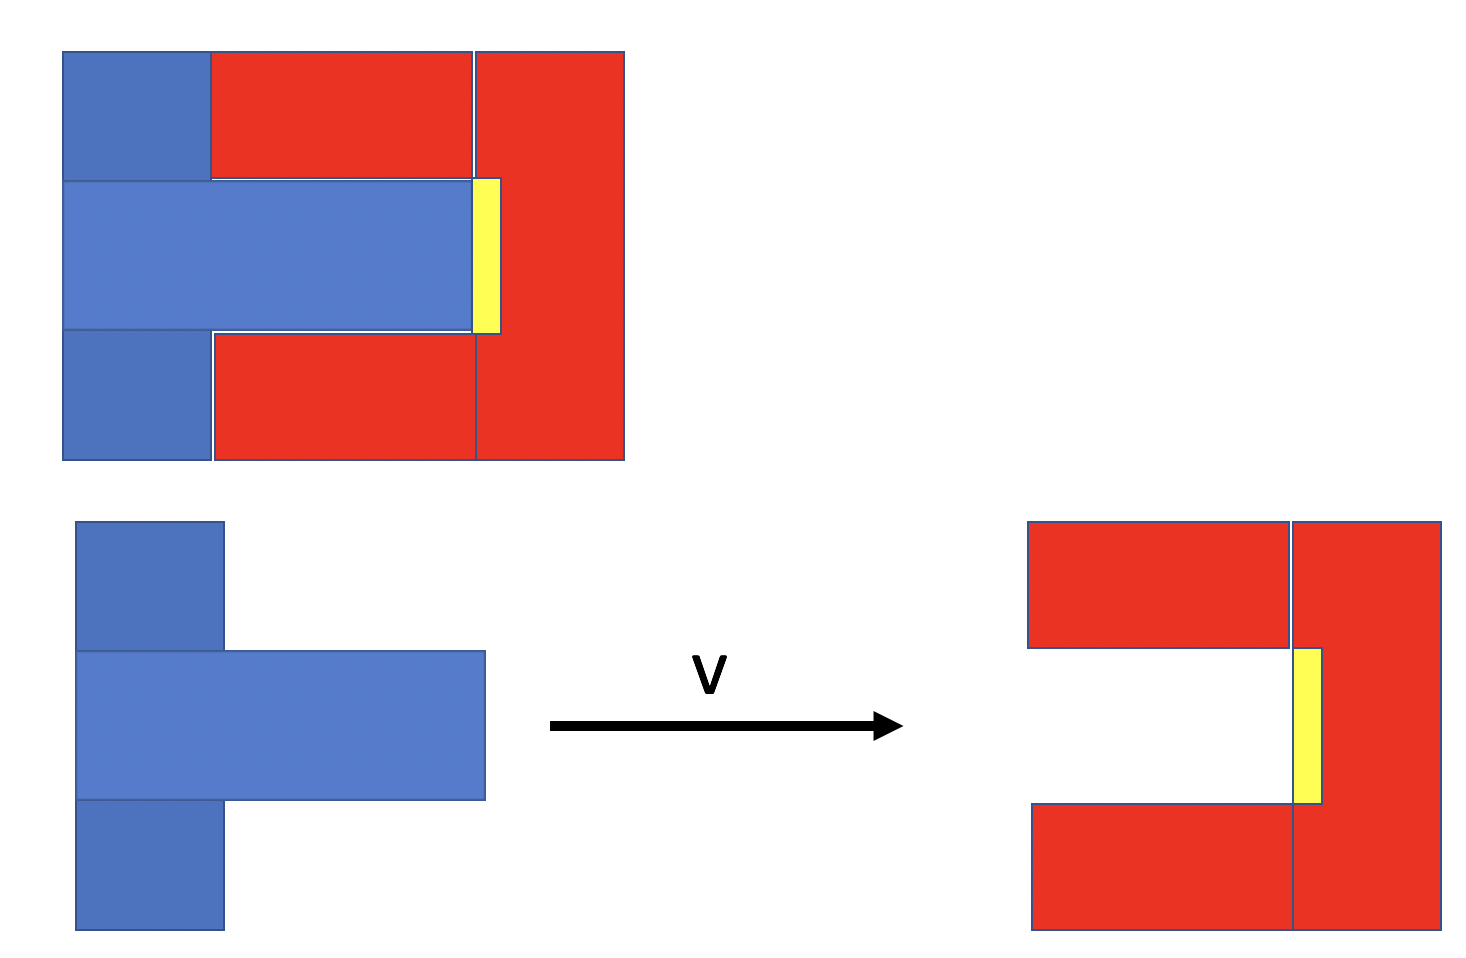
\includegraphics[scale=0.14]{media/detonator.png}}
Her ser du to innretninger, en blå og en rød. Øverst ser du de sammen og nederst så står den røde stille og den blå har høy hastighet rett mot den røde. Den gule boksen på den røde innretningen er en utløser for en bombe. Hvis den blå innretningen trykker på denne utløseren eksploderer bomben. Merk at i figuren øverst så er de ikke nærme nok til at bomba eksploderer. Tuppen av den blå må komme enda lenger inn. {\bf Husk lengdekontraksjon: når vi ser et legeme har en gitt hastighet så blir lengden av dette legemet mindre!}. \textcolor{blue}{Hvordan ser dette ut fra blått sitt referansesystem? Blir ikke rød da kortere og blå kan komme inn og utløse bomben?} \textcolor{red}{Og fra rødt sitt referansesystem? Blir ikke da den blåe enda kortere og kan ikke klare å utløse bomben?} {\bf Blir bomben utløst eller blir den ikke?} Sorry, du får ikke svaret her...
}{SIDE 56/56/56}

\begin{frame}
\label{oppsummering}
\hyperlink{pe20}{\pagebutton{\small Forrige side}}\href{https://nettskjema.no/a/171403}{\Changey[1][yellow]{2} \Changey[1][yellow]{-2}}
{\tiny
{\bf Du er ferdig med forelesning 2 av 2 i del 2B.} Du bør nå:
\begin{itemize}
\item vite hva verdenslinjer er og kunne tegne en verdenslinje for et legeme gitt hastigheten som funksjon av tiden
\item kunne utlede Newtons 1.lov fra prinsippet om maksimal aldring
\item vite hva en 4-vektor er og hvordan den transformerer mellom systemer
\item kunne utlede regneregler for 4-vektorer
\item kjenne Einsteins summekonvensjon, skalarprodukt og hvordan finne lengden av en 4-vektor.
\item kjenne uttrykket for 4-hastighet og kunne bruke dette til å transformere hastigheter fra et referansesystem til et annet
\item kjenne uttrykket for 4-bevegelsemengde og kunne tolke komponentene av denne, også for fotoner.
\item kunne utlede transformasjonen av energi og bevegelsemengde fra et referansesystem til et annet.
\item kunne utlede og bruke sammenhengen mellom relativistisk energi, bevegelsemengde og masse
\item kunne regne om energi og bevegelsesmengde mellom relativistiske enheter og SI-enheter
\end{itemize}
\textcolor{red}{Flott hvis du nå kan klikke på smilefjesene over og fortelle hva du synes om dette interaktive forelesningsnotatet. Hva var bra og nøyaktig hva kan forbedres? All ris og ros mottaes med takk!} {\bf Det anbefales nå at du sjekker \href{https://www.uio.no/studier/emner/matnat/astro/AST2000/h21/undervisningsmateriell/kortsvarsoppgaver/del2b.pdf}{kortsvarsoppgavene} til del 2B for å kontrollere at du har forstått stoffet. Kan du svare på disse, blir det lettere å bruke kunnskapen din i oppgavene/prosjektet. Noen av disse kommer på eksamen.}
}
\end{frame}


\end{document}
